\section{Experimental Evaluation}
\label{sec:experiments}

We evaluate GRL-SNAM on two navigation benchmarks that share the same \emph{stagewise, local-sensing} interface but differ in dynamics: (i) deformable hyperelastic ring navigation in cluttered workspaces, and (ii) point-agent dungeon navigation derived from~\citet{liang2023context}. In both tasks, GRL-SNAM receives the state $q_t$, a stage-exit goal $g_t$, and obstacles within a local window; task-specific dynamics and energy terms instantiate the reduced Hamiltonian $\mathcal{H}$.

\subsection{Tasks and Environments}
\label{subsec:tasks}

\paragraph{Stagewise local sensor and mapping effort quantification.}
At time $t$, the agent observes obstacles intersecting a local window $\mathcal{W}(q_t)$ of size $2\hat d \times 2\hat d$ centered at $q_t$, and a stage signal (macro-cell index) with its current exit goal $g_t$ from a stage manager over a workspace tiling. We quantify sensing effort by the mapping ratio
\begin{equation}
\rho_{\mathrm{map}} \;:=\; \frac{\mathrm{area}\!\left(\bigcup_t \mathcal{W}(q_t)\right)}{L^2}.
\label{eq:mapping_ratio}
\end{equation}

\subsubsection{ Narrow-Gap Passing Navigation Task with a Hyperelastic Ring Robot}
\label{subsubsec:ring_task}

\paragraph{Environment.}
Each instance is a $[0,L]\times[0,L]$ workspace with procedurally sampled circular obstacles (positions/radii/density), spanning bottlenecks, zig-zag corridors, and cul-de-sacs. Start--goal pairs are sampled so that a deformable ring admits a collision-free solution, while a rigid disc of comparable size may not. We construct Train, {In distribution Test(\textbf{Test-ID}, matched statistics), and Out-of-distribution Test (\textbf{Test-OOD}, shifted gap/density) splits}.

\paragraph{Dynamics and interface.}
The robot is a reduced-order hyperelastic ring with Hamiltonian $\mathcal{H}(q,p)$. GRL-SNAM interacts only through $(q_t, g_t, \mathcal{W}(q_t))$ and the resulting generalized forces/coefficients; implementation details of the hyperelastic model are provided in Section.~\ref{app:hyperelastic_model}.

\paragraph{Reduced Hamiltonian used in this task.}
We use a reduced Hamiltonian whose potential combines a goal term toward $g_t$ and barrier terms from signed distances to locally observed obstacles, with dissipation/regularization. Context encoders predict coefficients $(\beta,\gamma,\alpha)$ that modulate these terms.

\subsubsection{ Dungeon Navigation via a Point-Nav system }
\label{subsubsec:dungeon_task}

\paragraph{Environment and dynamics.}
We use dungeon layouts from~\citet{liang2023context}. The agent is a point mass in continuous 2D with state $q_t$ (position; optionally velocity) and action $\mathbf{a}_t=[v_x,v_y]\in[-3,3]^2$. Collisions with walls are penalized/terminating; reaching the goal yields reward.

\paragraph{Observations (matched to the stagewise interface).}
A \texttt{StagewiseSensor} selects the active macro-cell and exposes its exit as the local goal $g_t$. An \texttt{ObstacleExtractor} fits circular obstacles to wall segments inside $\mathcal{W}(q_t)$, returning centers, radii, and a visibility mask. The observation concatenates stage-relative position, $g_t$, and the local obstacle set.

\paragraph{Use in evaluation.}
We instantiate GRL-SNAM with a simple quadratic goal energy and radial barrier energies from the extracted obstacles, and compare to PPO/TRPO/SAC under (i) full-episode long-horizon training and (ii) short-rollout stagewise training with the same observation/action interface as GRL-SNAM.

\subsubsection{Experimental Setups}

We justify our choice of predefined hyperparemeters for each task in \cref{tab:hyperparams} and further explain them in \ref{subsec:hyperparam}. Most parameters are learnable or sharable across tasks. Only when maps' scale and robot configurations vary shall one choose additional hyperparameters. Experiments are performed on one NVIDIA A100 GPU with 40 GB VRAM, using Linux operating system, and all networks are trained via PyTorch \citep{paszke2019pytorch} library. For RL baselines, we adapt PPO, SAC and TRPO algorithms provided in Stable-Baselines3 \citep{stable-baselines3} for comparison. 


\begin{table}[t]
\centering
\caption{Hyperparameter nomenclature and selection across experiments. \textbf{Default: fixed.}
Parameters marked \learn are learned/predicted by the meta-policy (softplus-enforced nonnegativity where applicable); parameters marked \pre are precomputed.}
\label{tab:hyperparams}
\setlength{\tabcolsep}{5pt}
\renewcommand{\arraystretch}{1.12}
\small
\begin{tabularx}{\linewidth}{@{}l l X l@{}}
\toprule
\textbf{Block} & \textbf{Symbol} & \textbf{Description} & \textbf{Value / Range} \\
\midrule

\rowcolor{gray!15}\multicolumn{4}{@{}l@{}}{\textit{Learned coefficients (variable-dimension $\zeta_t$)}} \\
Barrier & $\bm{\alpha}_j$\learn & Per-obstacle barrier weight & $\alpha_j \ge 0$ (softplus) \\
Goal & $\bm{\beta}$\learn & Goal attraction strength & $\beta \ge 0$ (softplus) \\
Damping & $\bm{\gamma}$\learn & Linear damping scale & $\gamma \ge 0$ (softplus) \\
\midrule

\rowcolor{gray!15}\multicolumn{4}{@{}l@{}}{\textit{Shared pipeline: loss \& optimization}} \\
Opt. & $\eta$ & Learning rate & $1\times 10^{-4}$--$3\times 10^{-4}$ \\
Loss & $w_{\text{traj}},\, w_{\text{vel}}$ & Position / velocity loss weights & $1.0,\;1.0$ \\
Loss & $w_{\text{fric}},\, w_{\text{multi}}$ & Damping / multi-start penalty & $0.1,\;0.5$ \\
Rollout & $H$ & Surrogate rollout horizon & $2$--$6$ steps \\
Test-time & $\lambda_{\text{prox}}$ & Proximal regularization & $10^{-3}$ \\
\midrule

\rowcolor{gray!15}\multicolumn{4}{@{}l@{}}{\textit{Shared pipeline: IPC barrier \& staging}} \\
Barrier & $\hat d$ & Barrier activation distance & $0.28$--$1.0$ \\
Barrier & $b(d)$ & $-(d-\hat d)^2\log(d/\hat d)$ & --- \\
Staging & $(W,H)$ & Stage window dimensions & $(2.6,\,2.0)$ \\
Staging & $\rho_{\text{overlap}}$ & Stage overlap ratio & $0.3$ \\
Geometry & $r_{\text{inflate}}$ & Obstacle inflation (tube radius) & $0.05$--$0.4$ \\
\midrule

\rowcolor{blue!8}\multicolumn{4}{@{}l@{}}{\textit{Hyperelastic ring: dynamics}} \\
Trans. & $M_{\vec{c}},\,\gamma_{\vec{c}}$ & Robot pose mass / damping & $1.5,\;4.0$ \\

Scale & $M_s,\,\gamma_s$ & Scale mass / damping & $1.0,\;2.0$ \\
Material & $k_{\text{bulk}}$ & Bulk modulus (area stiffness) & $1.5$ \\
\midrule

\rowcolor{blue!8}\multicolumn{4}{@{}l@{}}{\textit{Hyperelastic ring: geometry}} \\
Shape & $r_{\text{robot}}$ & Nominal ring radius & $0.30$--$0.50$ \\
Spline & $n_{\text{ctrl}},\,K$ & B-spline control / sample points & $20,\;240$ \\
Time & $\Delta t$ & Integration timestep & $0.03$ \\
\midrule

\rowcolor{green!8}\multicolumn{4}{@{}l@{}}{\textit{Dungeon: FPE navigation}} \\
Speed & $v_{\max}$ & Maximum velocity & $2.5$--$3.0$ \\
Goal & $k_{\text{goal}}$ & Goal attraction gain & $20.0$--$25.0$ \\
Barrier & $k_{\text{barrier}}$ & Barrier repulsion gain & $0.0$ \\
Time & $\Delta t$ & Integration timestep & $0.3$ \\
\midrule

\rowcolor{green!8}\multicolumn{4}{@{}l@{}}{\textit{Dungeon: environment}} \\
Map & $\mathrm{SDF}(x,y)$\pre & Signed distance field (from grid) & --- \\
Staging & $s_{\text{stage}}$ & Stage window size & $60$ px \\
Waypoints & $d_{\text{wp}}$ & Minimum waypoint wall clearance & $1.5$--$4.0$ px \\
\bottomrule
\end{tabularx}
\end{table}




\subsection{Baseline Methods}
\label{subsec:baselines}

We compare GRL-SNAM against a spectrum of planning and learning methods that differ in (i) map access (full vs.\ local), (ii) planning scope (global vs.\ local), and (iii) supervision signal (hand-crafted surrogates vs.\ learned policies). Below we summarize the baselines and their roles.

\subsubsection{Baselines for Hyperelastic Ring Navigation}
\label{subsubsec:baselines_ring}

For the deformable hyperring task we consider two non-learning families plus our GRL-SNAM controller, all instantiated on the same hyperelastic model.

\paragraph{Global planners (full-map references).}
Assuming full occupancy grids, these methods provide reference paths and define $L_{\mathrm{ref}}$ for SPL and detour:
\begin{itemize}
    \item \textbf{Rigid A$^{\star}$:} A$^{\star}$ on an obstacle-inflated grid for a rigid disc of radius $r_{\text{rest}}$, yielding conservative collision-free paths that may be overly cautious for a deformable ring.
    \item \textbf{Deformable A$^{\star}$:} Clearance-aware A$^{\star}$ that augments edge costs with a deformation penalty as clearance approaches a minimum radius $r_{\min}$, allowing squeezing through tight passages at an energetic cost.
\end{itemize}

\paragraph{Local reactive planners (stagewise, same information as GRL-SNAM).}
To provide fair local baselines, we instantiate classical controllers that share the \emph{same} stage manager and local window as GRL-SNAM:
\begin{itemize}
    \item \textbf{Potential Fields (PF, staged):} Attractive potential toward the current stage exit plus repulsive potentials from locally sensed obstacles and stage boundaries.
    \item \textbf{Control Barrier Functions (CBF, staged):} A nominal control toward the stage exit filtered through a CBF quadratic program using clearance-based barrier functions to enforce local safety.
    \item \textbf{Dynamic Window Approach (DWA, staged):} Sampling of $(v,\omega)$ pairs within dynamics limits, short-horizon rolling, and scoring based on goal alignment, velocity, and clearance with penalties for leaving the active stage.
\end{itemize}
All three operate under identical sensing and stagewise constraints as GRL-SNAM, but rely on hand-crafted surrogates instead of learned Hamiltonians.

\paragraph{Ours: GRL-SNAM (hyperring instantiation).}
On the hyperelastic ring, GRL-SNAM uses the reduced Hamiltonian described in Section~\ref{subsec:navigator_meta_learner} and ~\ref{app:hyperelastic_model}, combining goal, barrier, and dissipation terms with adaptive coefficients $(\beta,\gamma,\alpha)$ predicted by context encoders. It shares the same stage manager and local window as the reactive baselines but learns the local force field from short rollouts instead of fixing it a priori. All hyperring results (minimal sensing vs.\ navigation quality, planner comparisons, Hamiltonian field analysis, ablations, robustness) are reported against this set.

\subsubsection{Baselines for Dungeon Point-Agent Navigation}
\label{subsubsec:baselines_dungeon}

All dungeon methods share the same point-agent dynamics and action space, so differences reflect the planning/learning rule and map access (Fig.~\ref{fig:dungeon_map}).

\begin{figure}[h!]
    \centering
    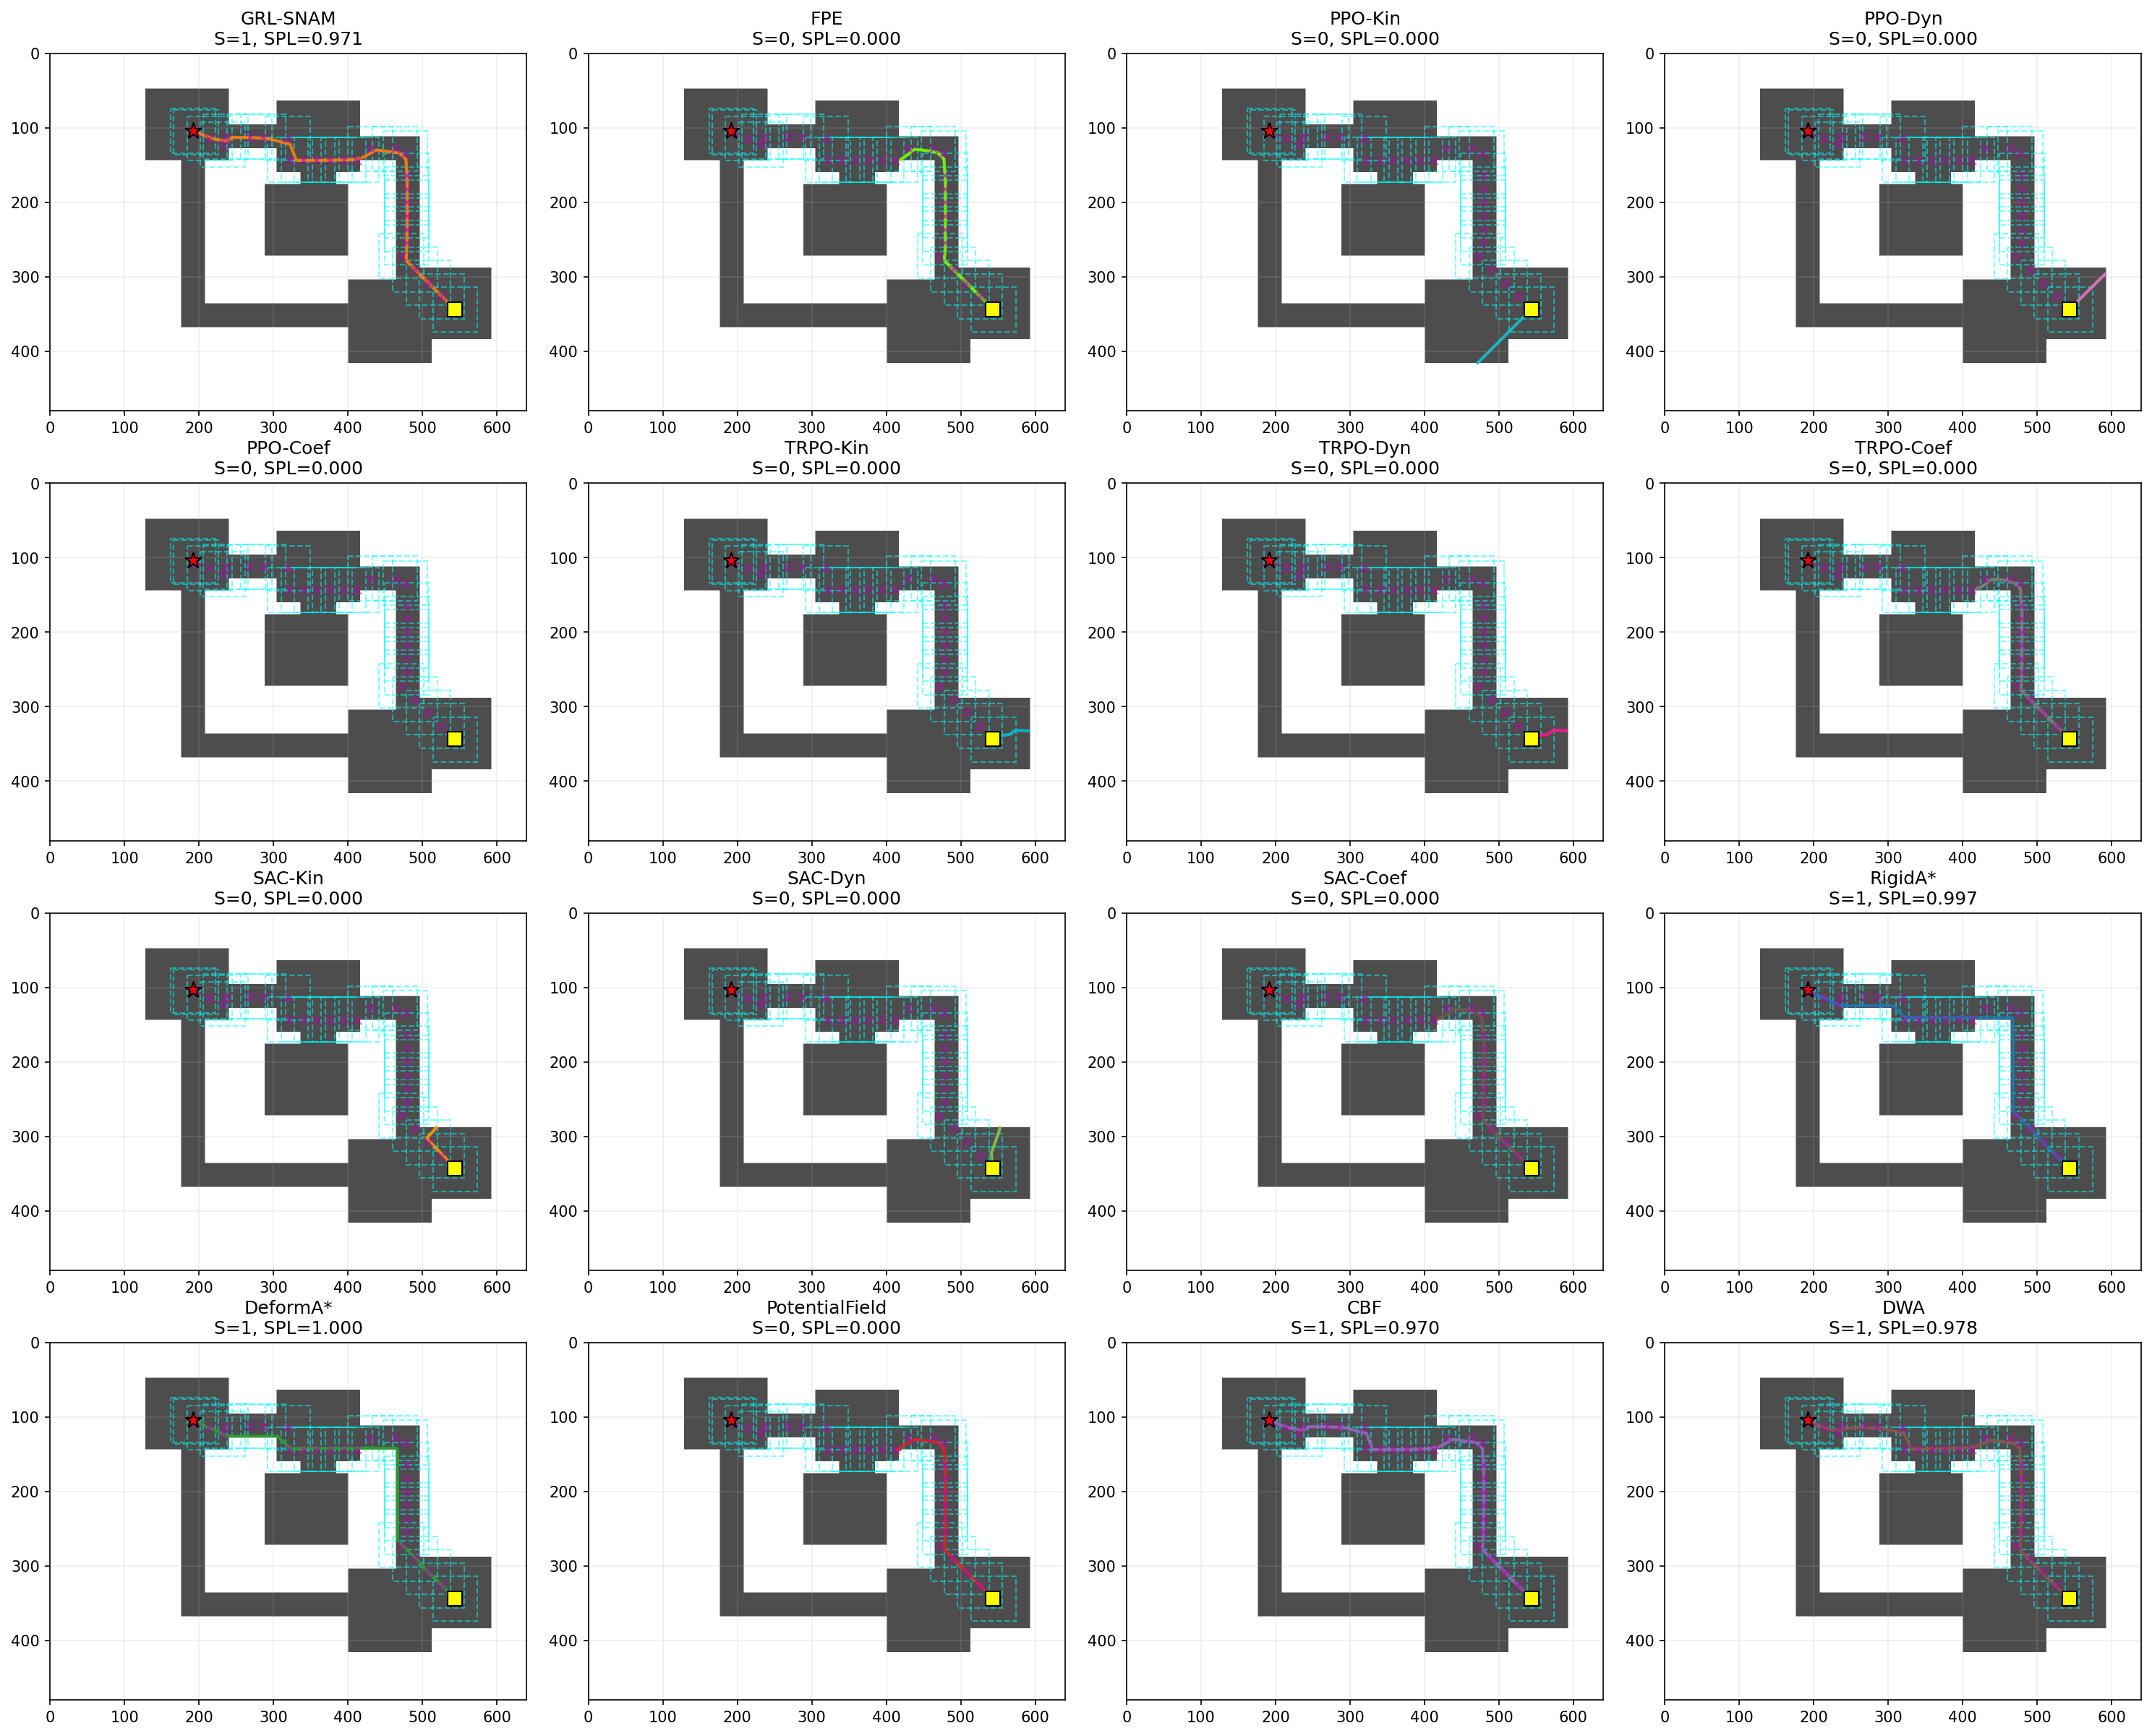
\includegraphics[width=\linewidth]{10_comparison.png}
    \caption{\textbf{Representative dungeon rollouts under stagewise local sensing.} Each panel shows the same layout with the goal (red $\times$), start (yellow square), executed trajectory (colored by time), and the union of visited sensing windows $\mathcal{W}(q_t)$ (cyan boxes). Panel titles report episode success $S$ and SPL (with Grid A$^{\star}$ as the reference path length $L_{\mathrm{ref}}$). GRL-SNAM reaches the goal with near-planner efficiency, whereas stagewise deep-RL baselines (PPO/TRPO/SAC with Kin/Dyn/Coef parameterizations) and the greedy potential-field baseline fail on this instance; classical planners and safety-filtered local methods (CBF/DWA) succeed but follow more conservative routes.}

    \label{fig:dungeon_map}
\end{figure}

\paragraph{Classical baselines.}
\begin{itemize}
    \item \textbf{Grid A$^{\star}$ (full map):} 8-connected A$^{\star}$ on the true occupancy grid; used as the path-length reference $L_{\mathrm{ref}}$.
    \item \textbf{Greedy PF (local):} moves toward the goal with repulsion from walls in the local occupancy patch.
    \item \textbf{Local DWA (local):} samples velocity commands $(v_x,v_y)$, rolls out short trajectories against locally sensed walls, and scores by goal alignment, clearance, and length.
\end{itemize}

\paragraph{Deep RL baselines.}
We train PPO~\citep{schulman2017ppo}, TRPO~\citep{schulman2015trust}, and SAC~\citep{haarnoja2018sac} with the same encoder and observation encoding under two regimes:
\begin{itemize}
    \item \textbf{Full-episode RL (long horizon):} standard end-to-end episodes with a global goal and a fixed step budget (e.g., 2000), without stage supervision.
    \item \textbf{Stagewise RL (short rollouts):} the same stagewise observation/action interface as GRL-SNAM: stage-relative state, stage-exit goal, and local extracted obstacles; episodes are extended to $K_{\mathrm{ext}}=8K$ to support exploration.
\end{itemize}

\paragraph{Within-framework variants (same data, different learning rule).}
Holding the stagewise interface and short-rollout dataset fixed, we replace Hamiltonian-structured supervision with:
\begin{itemize}
    \item \textbf{Velocity regression:} supervised prediction of $\mathbf{a}_t$ from observations.
    \item \textbf{Coefficient RL:} policy-gradient learning over Hamiltonian coefficients $(\alpha,\beta,\gamma)$ instead of the DfPO-style objective.
\end{itemize}


\subsection{Metrics and Evaluation Protocol}
\label{subsec:metrics_protocol}

Across both tasks we evaluate methods along four axes:
(i) task success and path efficiency,
(ii) safety and physical plausibility,
(iii) mapping / sensing budget, and
(iv) learning efficiency and robustness.
Unless stated otherwise, we report averages over multiple random seeds and environment instances.

\paragraph{Navigation performance.}
We report:
(i) \textbf{success rate} (fraction of episodes reaching the goal without hard collisions),
(ii) \textbf{Success-weighted Path Length (SPL)}, measuring path efficiency relative to a reference planner (Rigid A$^{\star}$ for hyperring, Grid A$^{\star}$ for dungeon),
and (iii) \textbf{detour ratio} $L / L_{\mathrm{ref}}$ over successful runs, indicating excess path length relative to the reference. We also track \textbf{smoothness} via average heading change per step to assess physical plausibility.

\paragraph{Safety and clearance.}
Safety is quantified by the \textbf{minimum} and \textbf{mean clearance} to the nearest obstacle along a trajectory (positive values indicate safety margins, negative values indicate penetrations), the number of \textbf{hard collisions} per episode, and, for methods with explicit barriers (CBF, GRL-SNAM, Deformable A$^{\star}$), the fraction of timesteps that violate a prescribed safety threshold (barrier violations).

\paragraph{Mapping and sensing budget.}
To measure how much of the environment each method must observe, we define the \textbf{mapping ratio} as the fraction of workspace area that ever falls inside a local sensing window during an episode. All stagewise methods (PF, CBF, DWA, GRL-SNAM, dungeon local baselines) use the same window size $2\hat d \times 2\hat d$; global planners (Rigid A$^{\star}$, Grid A$^{\star}$) have mapping ratio $100\%$.

\paragraph{Learning efficiency.}
For learning-based methods (GRL-SNAM, deep RL, within-framework variants) we track \textbf{sample efficiency} via success and SPL as functions of training interaction steps, summarize performance with area under the learning curve, and report the steps required to reach target thresholds (e.g., $80\%$ success or SPL $\geq 0.7$). For GRL-SNAM, “steps’’ are short-rollout samples used in supervised Hamiltonian training; for PPO/TRPO/SAC they are environment transitions. We also report total environment steps, gradient updates, and update-to-sample ratios where relevant.

\paragraph{Evaluation protocols.}
For hyperelastic ring experiments, each environment is evaluated from multiple random start–goal pairs (typically $50$), and we report aggregated statistics on Test-ID and Test-OOD splits. Unless noted, navigation-quality tables (e.g., Table~\ref{tab:success_only}) are computed on \emph{successful runs only} to isolate path quality from outright failure. For dungeon experiments, full-episode baselines are trained and evaluated on long-horizon episodes with fixed step budgets, while short-rollout baselines and GRL-SNAM are trained on a stagewise dataset with horizon $H \in [2,6]$ and evaluated on a held-out set of stagewise test samples with identical observation and action spaces. Robustness experiments vary sensing and dynamics fidelity over a grid of perturbation levels (e.g., position jitter, radius errors, missed/false obstacles, damping perturbations) and report success, SPL, clearance, and collisions; ablations vary only the training objective while keeping environments fixed, reporting the same core metrics plus qualitative behavior summaries.

% ========================================================

\subsection{Results at a Glance}
\label{subsec:results_overview}

Across the hyperelastic ring and dungeon point-agent tasks, results support four takeaways:

\begin{enumerate}
    \item { Effective Path Planning under minimal sensing}
    On the hyperelastic ring, GRL-SNAM attains CBF-level efficiency while observing only sparse stagewise windows: Table~\ref{tab:success_only} shows SPL $\approx 0.95$ and detour $\approx 1.09$ at a mapping ratio of $\sim$10--11\%, comparable to PF's sensing budget but with substantially higher path efficiency.

    \item \textbf{Stronger navigation than {conventional, reactive, and deep RL baselines.}}
    On ring Test-ID/OOD, GRL-SNAM achieves near-perfect success with high SPL, smooth trajectories, and positive clearance, while A$^{\star}$ planners, PF/CBF/DWA, and RL baselines trade off safety vs.\ efficiency or fail in clutter (Fig.~\ref{fig:exp1_paths}, Fig.~\ref{fig:exp1_comparison}). In the dungeon benchmark, GRL-SNAM substantially outperforms PPO/TRPO/SAC trained end-to-end over millions of steps, and also outperforms their stagewise short-rollout versions under the same observation/action interface (Table~\ref{tab:full_episode_rl}, Table~\ref{tab:short_rollout_rl}).

    \item \textbf{The gain comes from the { adaptive reward and geometric Hamiltonian learning.}}
    Under matched stagewise sensing and short-rollout data, PPO/TRPO/SAC plateau below $30\%$ success, whereas GRL-SNAM reaches $\sim$90\% success with $\sim$500k supervised updates on the same interface (Table~\ref{tab:short_rollout_rl}), indicating the advantage is driven by Hamiltonian-structured supervision rather than algorithm choice.

    \item \textbf{Interpretable fields, learned constraints, and robust adaptation.}
    GRL-SNAM learns a coherent force field that balances goal attraction and barrier repulsion via adaptive coefficients $(\beta,\gamma,\alpha)$ (Fig.~\ref{fig:vector_fields}, Fig.~\ref{fig:time_series}) and recovers barrier-like energy profiles from interaction (Fig.~\ref{fig:barrier_profile}). Ablations isolate the role of dissipation and near-contact training (Table~\ref{tab:ablation_fric_multi}), and robustness tests show graceful degradation under sensing/dynamics noise (Table~\ref{tab:robustness}). Replay analysis indicates the system stores compact local transitions and constraint summaries rather than full maps (Fig.~\ref{fig:replay_buffer}).
\end{enumerate}

We next quantify sensing--performance trade-offs, then present the main ring and dungeon comparisons, followed by field analyses, ablations, and robustness.

\subsection{Navigation Quality vs.\ Mapping Effort under Minimal Sensing}
\label{subsec:minimal_sensing}

We test whether GRL-SNAM can achieve near-planner navigation while sensing only a small fraction of the workspace. {The dataset contains all the noise levels mentioned in \cref{tab:robustness}}
All \emph{stagewise} methods share the same stage manager and local sensing window of size $2\hat d \times 2\hat d$; they differ only in how local observations are converted into forces/actions. We compare (i) classical local controllers (PF, CBF), (ii) GRL-SNAM, and (iii) deep RL trained under the \emph{same} stagewise sensing and short-rollout distribution as GRL-SNAM.

\paragraph{RL under matched interfaces.}
For PPO, TRPO, and SAC we evaluate three control parameterizations:
\textbf{Kin} (output velocities), \textbf{Dyn} (output forces integrated by a damped point-mass model), and \textbf{Coef} (output Hamiltonian coefficients $(\alpha,\beta,\gamma)$). 
Thus, RL baselines share observations, local dynamics, and Hamiltonian building blocks with GRL-SNAM; only the learning rule and control parameterization change.

\paragraph{Metrics.}
On \emph{successful runs} we report SPL, detour $L/L_{\mathrm{ref}}$ (Rigid A$^{\star}$ reference), minimum clearance (negative indicates penetration), and mapping ratio (fraction of workspace covered by any sensing window).

\begin{table}[h!]
\centering
\caption{Navigation quality vs.\ mapping effort on the hyperelastic ring task (success-only runs). 
All stagewise methods use the same sensing window and stage manager. RL variants share the same stagewise sensing and short-rollout distribution as GRL-SNAM, differing only in control parameterization (Kin/Dyn/Coef) and learning rule.}
\vspace{0.4em}
\begin{tabular}{lcccc}
\toprule
Method       & SPL $\uparrow$ & Detour $\downarrow$ & MinClear (m) $\uparrow$ & Mapping (\%) $\downarrow$ \\
\midrule
PF           & 0.77     & 1.42 & 0.18           & 10.3 \\
CBF          & \textbf{0.96}     & \textbf{1.04} & \textbf{0.32}  & 11.2 \\
GRL-SNAM     & \textit{0.95} & \textit{1.09} & \textit{0.26} & \textbf{10.7} \\
\midrule
PPO-Kin      & 0.143    & 1.87 & $-0.358$       & 15.4 \\
PPO-Dyn      & 0.000    & 2.31 & 0.771          & 18.1 \\
PPO-Coef     & 0.071    & 1.65 & $-0.092$       & 14.7 \\
TRPO-Kin     & 0.000    & 2.12 & $-0.327$       & 16.5 \\
TRPO-Dyn     & 0.000    & 1.98 & 0.019          & 15.9 \\
TRPO-Coef    & 0.571    & 1.44 & 0.004          & 15.3 \\
SAC-Kin      & 0.000    & 2.27 & $-0.229$       & 16.8 \\
SAC-Dyn      & 0.000    & 2.41 & $-0.229$       & 16.9 \\
SAC-Coef     & 0.571    & 1.53 & 0.004          & 14.6 \\
\bottomrule
\end{tabular}
\label{tab:success_only}
\end{table}

\paragraph{Near-planner quality at minimal mapping.}
Table~\ref{tab:success_only} shows that GRL-SNAM matches CBF-level efficiency (SPL $0.95$ vs.\ $0.96$; detour $1.09$ vs.\ $1.04$) while requiring essentially the same mapping ratio as PF ($10.7\%$ vs.\ $10.3\%$). 
PF, despite identical sensing, yields substantially longer paths (detour $1.42$) and lower SPL ($0.77$), indicating that the improvement comes from how sensed patches are converted into a local navigation field, not from sensing more of the map.

\paragraph{RL does not close the gap under matched sensing.}
Deep RL variants consume \emph{more} mapping (typically $14$--$18\%$) yet remain far behind GRL-SNAM. We observe three recurring behaviors:
(i) \textbf{Kin} policies often graze or collide (negative MinClear) and achieve low SPL; 
(ii) \textbf{Dyn} policies frequently stall or fail to complete (near-zero SPL, large detours); and 
(iii) \textbf{Coef} policies are strongest (TRPO/SAC-Coef), but still require higher mapping and operate at near-grazing clearances ($\approx 0.004$m) with only moderate SPL ($0.57$). 
Changing optimizer (PPO/TRPO/SAC) or parameterization (Kin/Dyn/Coef) shifts outcomes but does not reproduce the efficiency--safety trade-off achieved by GRL-SNAM.

\paragraph{Takeaway.}
Under identical stagewise sensing, GRL-SNAM is the only method that simultaneously attains high path efficiency (near CBF), low mapping (near PF), and strictly positive clearance, suggesting the main advantage is the Hamiltonian-structured supervision that learns a constraint-aware local energy landscape rather than a direct reward-maximizing policy.


\subsection{Comprehensive Navigation Comparison}
\label{subsec:comprehensive_nav}

We compare GRL-SNAM to (i) full-map global planners (Rigid A$^{\star}$, Deformable A$^{\star}$), 
(ii) stagewise local controllers (PF, CBF, DWA) with the same sensing window and stage manager, 
and (iii) deep RL policies trained under the same stagewise, short-rollout interface as GRL-SNAM (Kin/Dyn/Coef).
We evaluate on Test-ID and Test-OOD using success, SPL, detour $L/L_{\mathrm{ref}}$, minimum clearance, and smoothness.
Figure~\ref{fig:exp1_comparison} reports aggregate metrics and Figure~\ref{fig:exp1_paths} shows representative rollouts.

\paragraph{Performance across ID and OOD.}
GRL-SNAM maintains near-perfect success on both Test-ID and Test-OOD and achieves the highest SPL with low variance.
By contrast, full-map planners are either conservative (inflation-induced detours) or sensitive to hand-tuned deformation costs, and stagewise reactive methods (PF/CBF/DWA) degrade on Test-OOD due to local oscillations, stalls, or cul-de-sac behavior.

\paragraph{Aggregate trade-offs (readout of Fig.~\ref{fig:exp1_comparison}).}
{Fig.~\ref{fig:exp1_comparison} is organized as two dashboards: Test-ID (left) and Test-OOD (right).
Within each dashboard, the \emph{top row} reports task-level performance and efficiency:
(\textit{left}) success rate (fraction of episodes reaching the goal),
(\textit{middle}) the distribution of SPL (zeros indicate failures; values near one indicate near-shortest successful paths),
and (\textit{right}) average path length, which disambiguates whether high SPL comes from genuinely short paths versus a small number of efficient successes.
The \emph{bottom row} reports safety and cost:
(\textit{left}) the distribution of per-episode minimum clearance
$\mathrm{clr}_{\min}=\min_n \mathrm{clr}_n$ (lower tails indicate grazing/collisions),
(\textit{middle}) the “grazing rate” $\mathbb{P}(\mathrm{clr}_{\min}\le d_{\text{thr}})$ for a fixed threshold $d_{\text{thr}}$ (here $1.5$),
and (\textit{right}) average computation time per episode.

Across both Test-ID and Test-OOD, GRL-SNAM couples \emph{high success} with an SPL distribution concentrated near high values, while maintaining strictly positive clearance (small lower tail and low grazing rate).
In contrast, kinematic/dynamic RL baselines show a larger mass at low SPL (more failures and inefficient successes) and heavier low-clearance tails, while conservative/global planners and potential-field variants tend to keep large clearance but pay for it with reduced efficiency (lower SPL / longer paths) and, in some settings, additional failures from overly conservative detours or local minima.}

\paragraph{Qualitative behavior.}
{Fig.~\ref{fig:exp1_paths} shows a representative \emph{Test-OOD bottleneck} layout (start: $\star$, goal: $\square$; circles: obstacles). Each panel title reports \emph{Success} and \emph{SPL}.
\textbf{Row 1 (GRL-SNAM and PPO variants):}
GRL-SNAM (top-left) executes a single, smooth \emph{squeeze-and-recover} maneuver: it threads the narrow gap between the upper obstacle cluster and the large central obstacle, then recenters and reaches the goal with minimal detour (Success $=1$, SPL $=1$). In contrast, PPO-Kin and PPO-Dyn (top row, middle) fail in this bottleneck: the kinematic variant stalls short of the goal, while the dynamic variant drifts into an unproductive detour and times out (Success $=0$). PPO-Coef (top-right) illustrates that even when coefficients are learnable, the rollout can still fail on this OOD geometry (Success $=0$), reflecting sensitivity to tight clearances.

\textbf{Row 2 (TRPO variants and SAC-Kin):}
TRPO-Kin and TRPO-Dyn (second row, left/middle) again fail to traverse the bottleneck (Success $=0$), typically stopping early or clipping the corridor geometry. TRPO-Coef (second row, third) succeeds (Success $=1$) but the path \emph{hugs obstacle boundaries} through the constriction, indicating smaller clearance margins than GRL-SNAM. SAC-Kin (second row, right) also fails on this instance (Success $=0$).

\textbf{Row 3 (SAC variants and global planners):}
SAC-Dyn (third row, left) fails (Success $=0$) and exhibits a large, boxy detour pattern that does not resolve the bottleneck. SAC-Coef (third row, second) succeeds (Success $=1$) but, similar to TRPO-Coef, succeeds by skimming close to obstacles in the narrow passage. The global planners RigidA* and DeformA* (third row, right two panels) both succeed (Success $=1$) but produce \emph{piecewise-linear and/or conservative} routes with multiple right-angle turns and larger stand-off distances, yielding longer paths that avoid exploiting the short near-boundary squeeze.

\textbf{Row 4 (classical local controllers):}
Potential Field (bottom-left) fails (Success $=0$), consistent with a local-minimum/trapping failure mode near the bottleneck. By contrast, CBF and DWA (bottom-middle/right) both succeed (Success $=1$), but their rollouts show characteristic \emph{reactive behavior}: visible curvature/adjustments around obstacles and a less direct route than GRL-SNAM, reflecting oscillations or conservative arcs induced by local constraint satisfaction.}

Global planners succeed but generate jagged { or overly conservative paths that does not exploit near boundary squeezing path which can be shorter}.

\begin{figure}[h!]
    \centering
    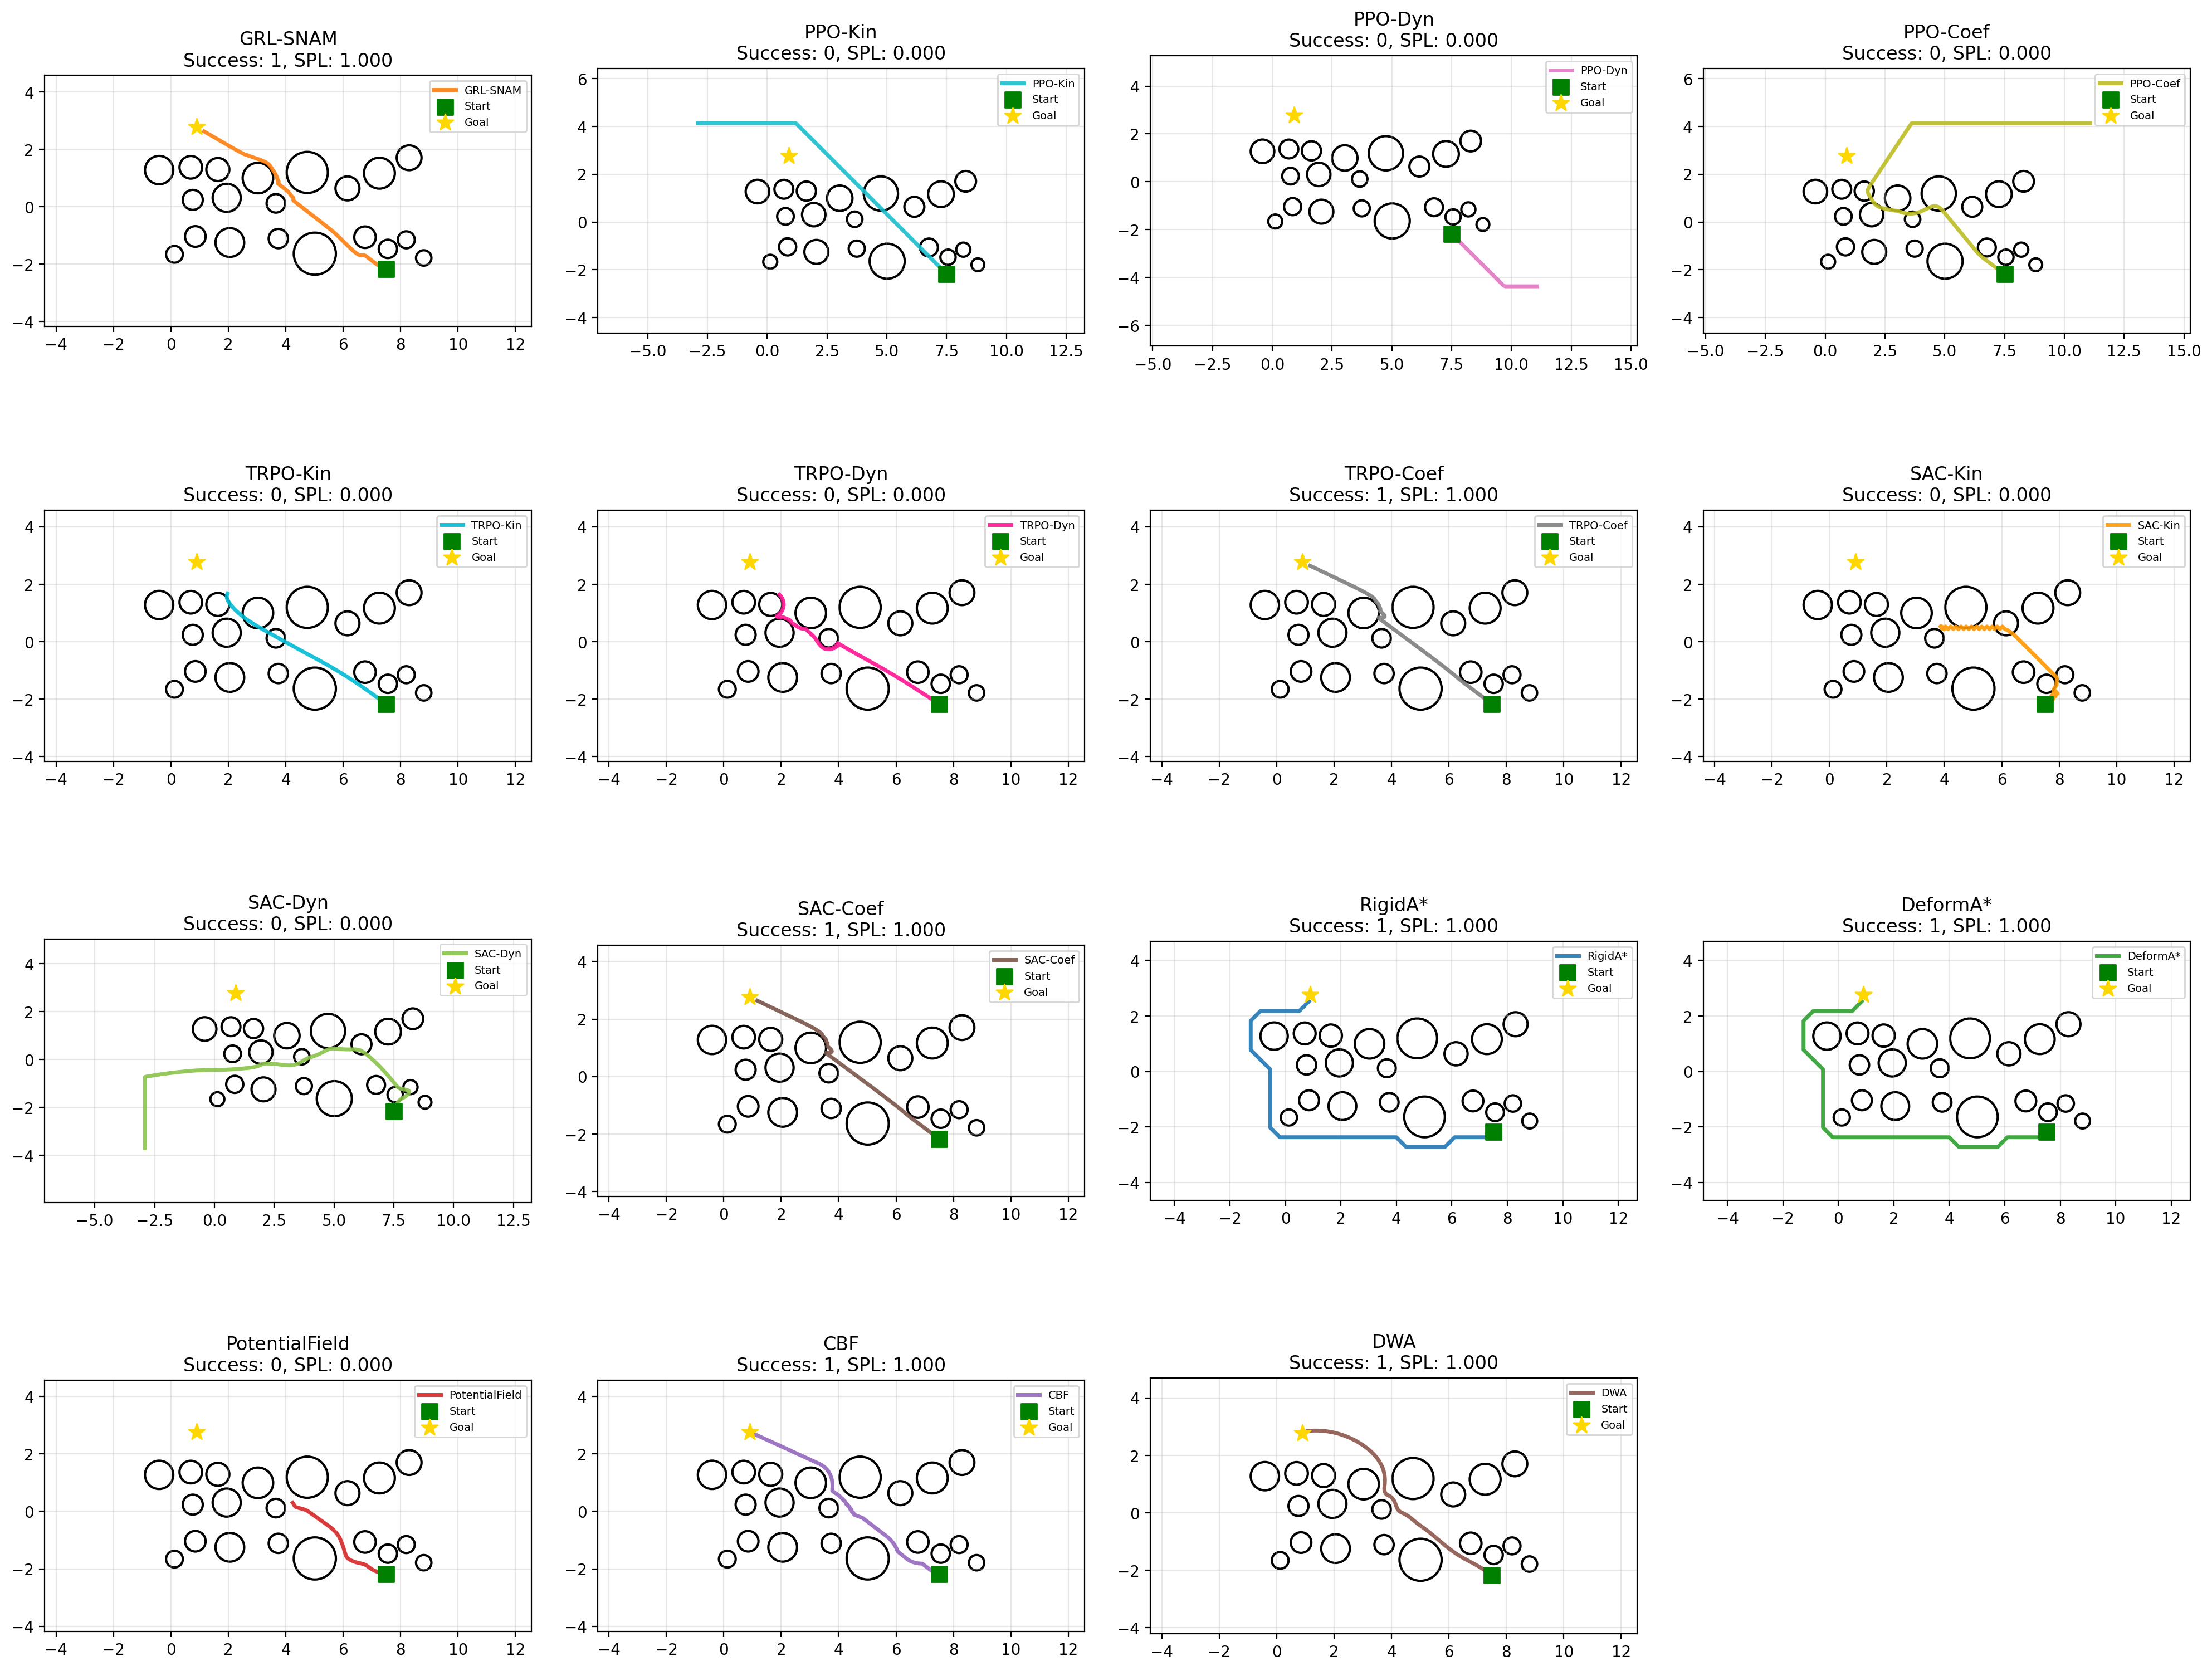
\includegraphics[width=\linewidth]{comprehensive_comparison.png}
    \caption{{\textbf{Qualitative rollouts on a representative Test-OOD bottleneck layout.} Start is marked by $\star$, goal by $\square$, and circles denote obstacles; each panel title reports Success and SPL. \textbf{Row 1:} GRL-SNAM and PPO (Kin/Dyn/Coef). \textbf{Row 2:} TRPO (Kin/Dyn/Coef) and SAC-Kin. \textbf{Row 3:} SAC (Dyn/Coef) and global planners (RigidA*, DeformA*). \textbf{Row 4:} classical local methods (Potential Field, CBF, DWA). GRL-SNAM is the only method here that achieves a smooth, short \emph{squeeze-and-recover} trajectory through the bottleneck without grazing, while learning-based baselines either fail (Kin/Dyn) or succeed by boundary-hugging (Coef). Global planners succeed but are jagged/overly conservative, and local controllers highlight reactive artifacts (trapping for PF; oscillatory/arc-like adjustments for CBF/DWA).}}


    \label{fig:exp1_paths}
\end{figure}

\begin{figure}[h!]
    \centering
    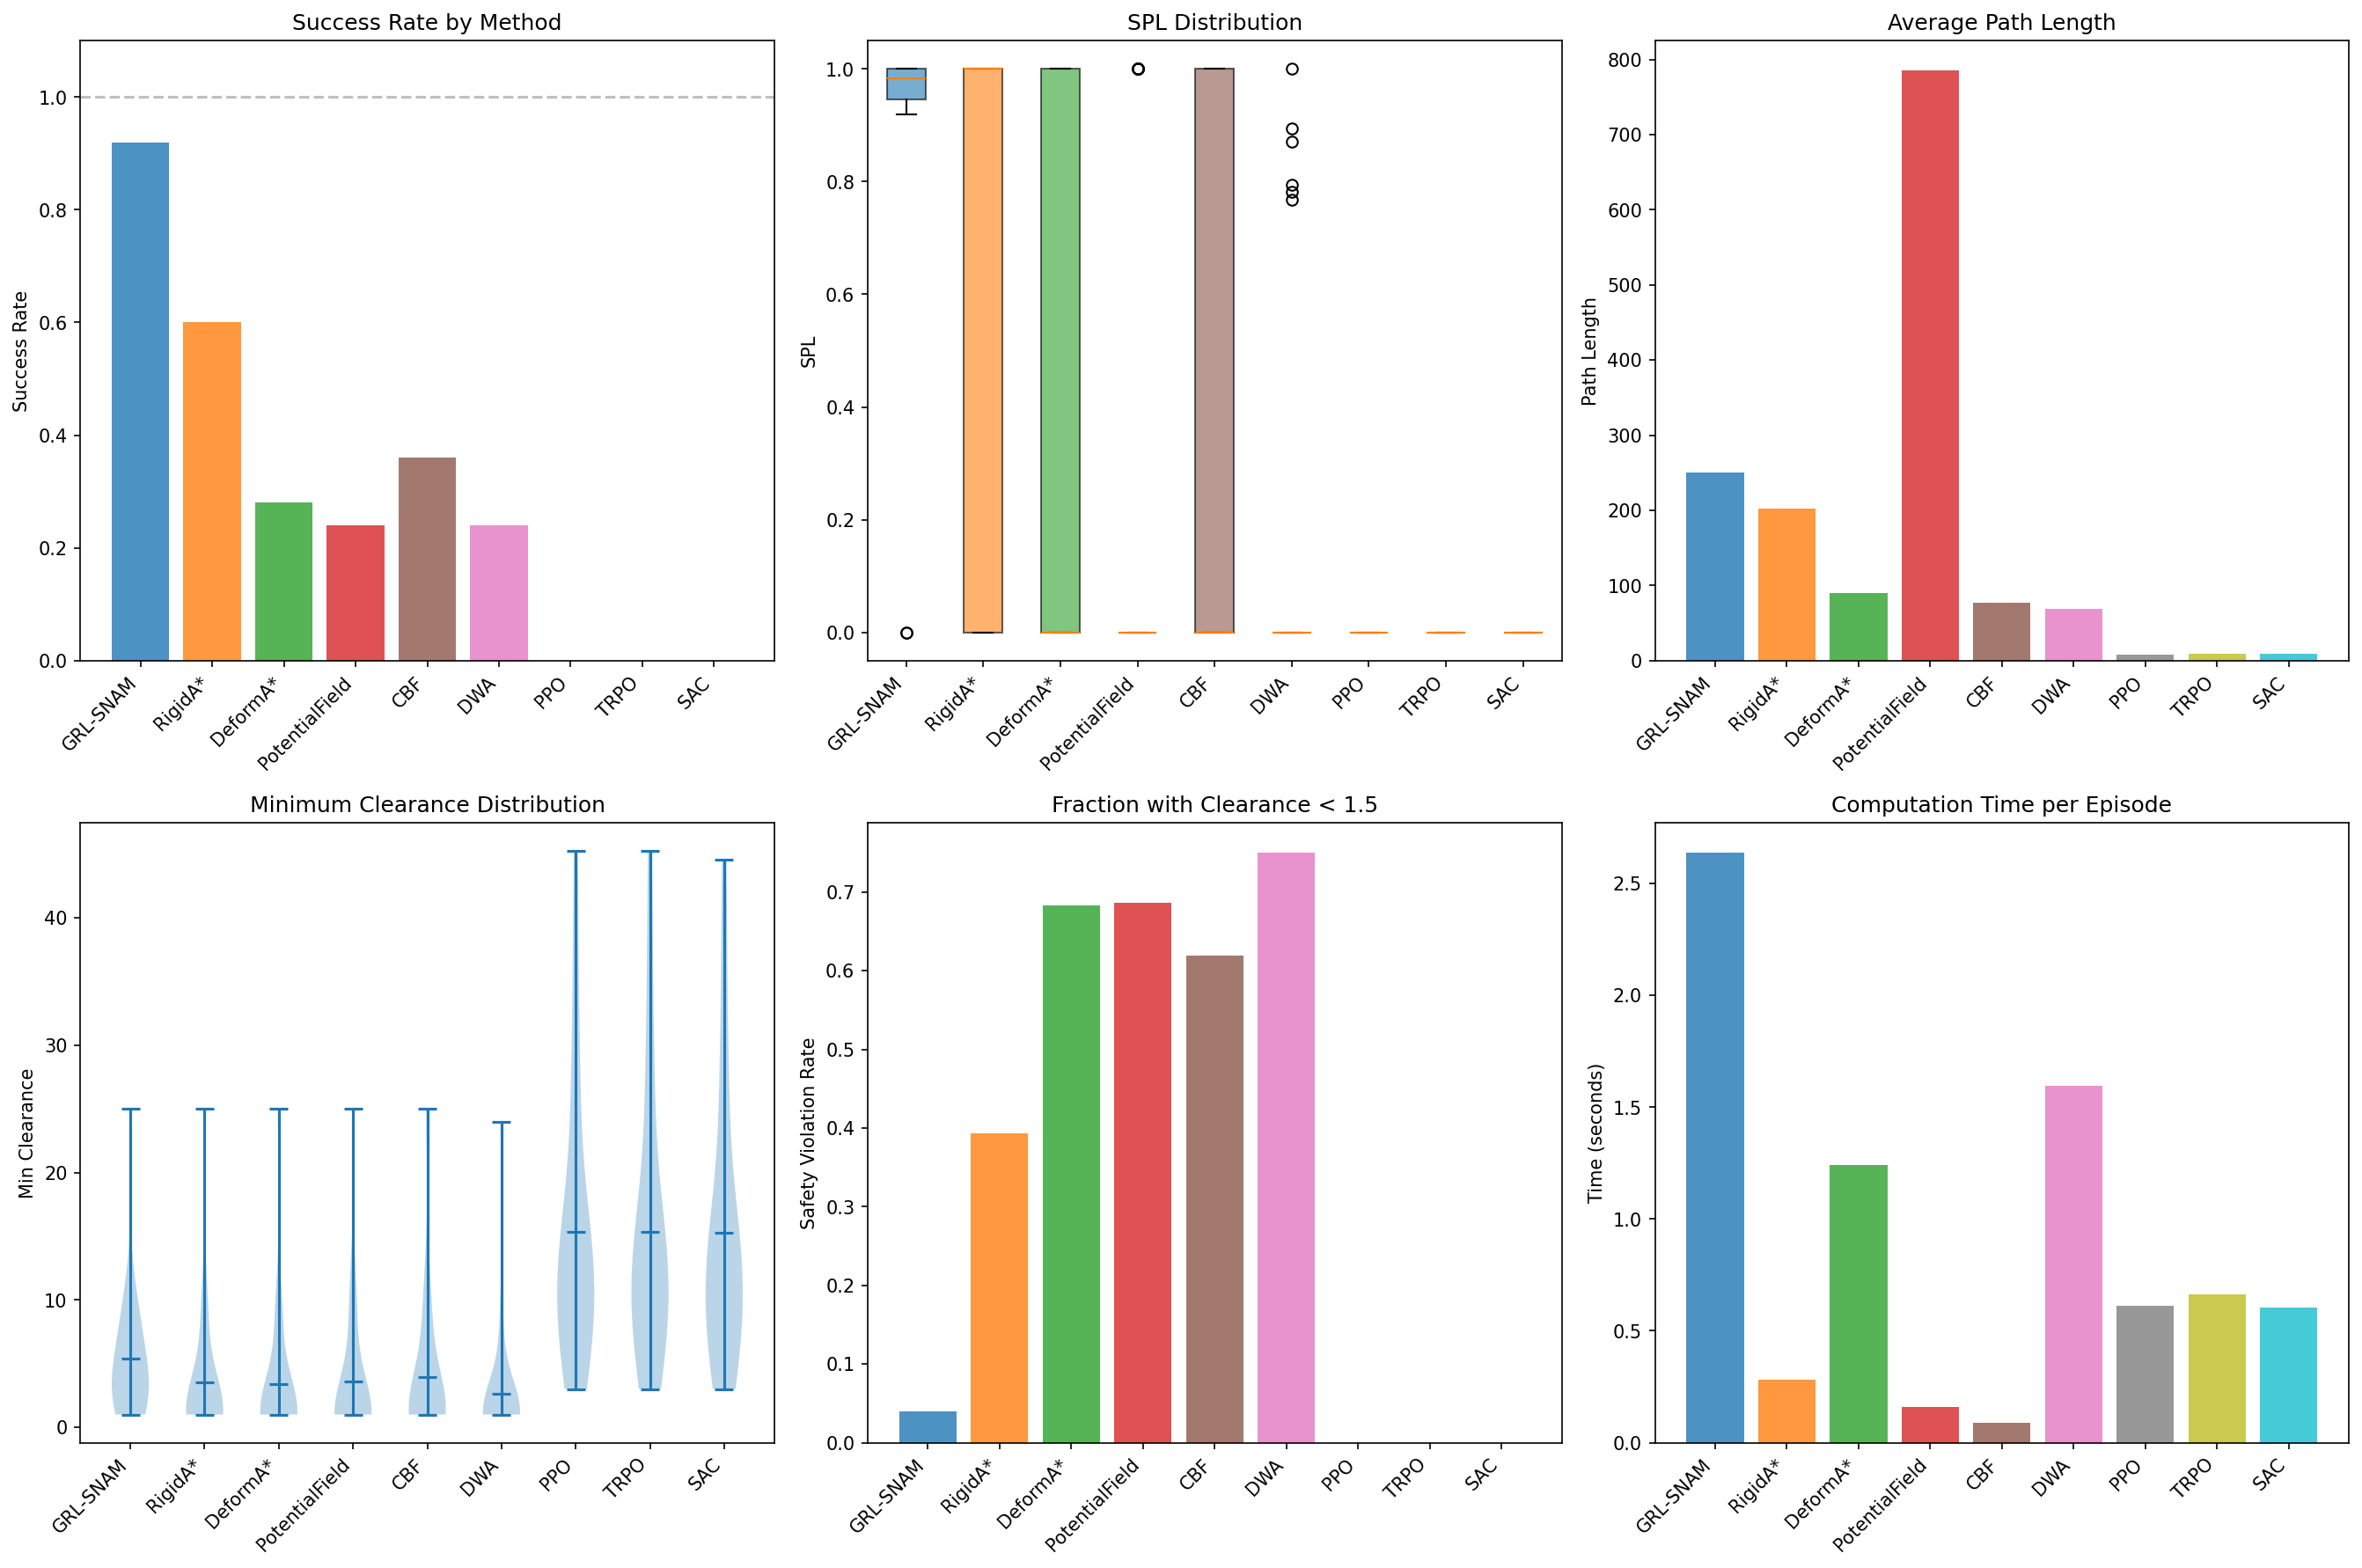
\includegraphics[width=0.48\linewidth]{AllTrials_dashboard.png}
    \hfill
    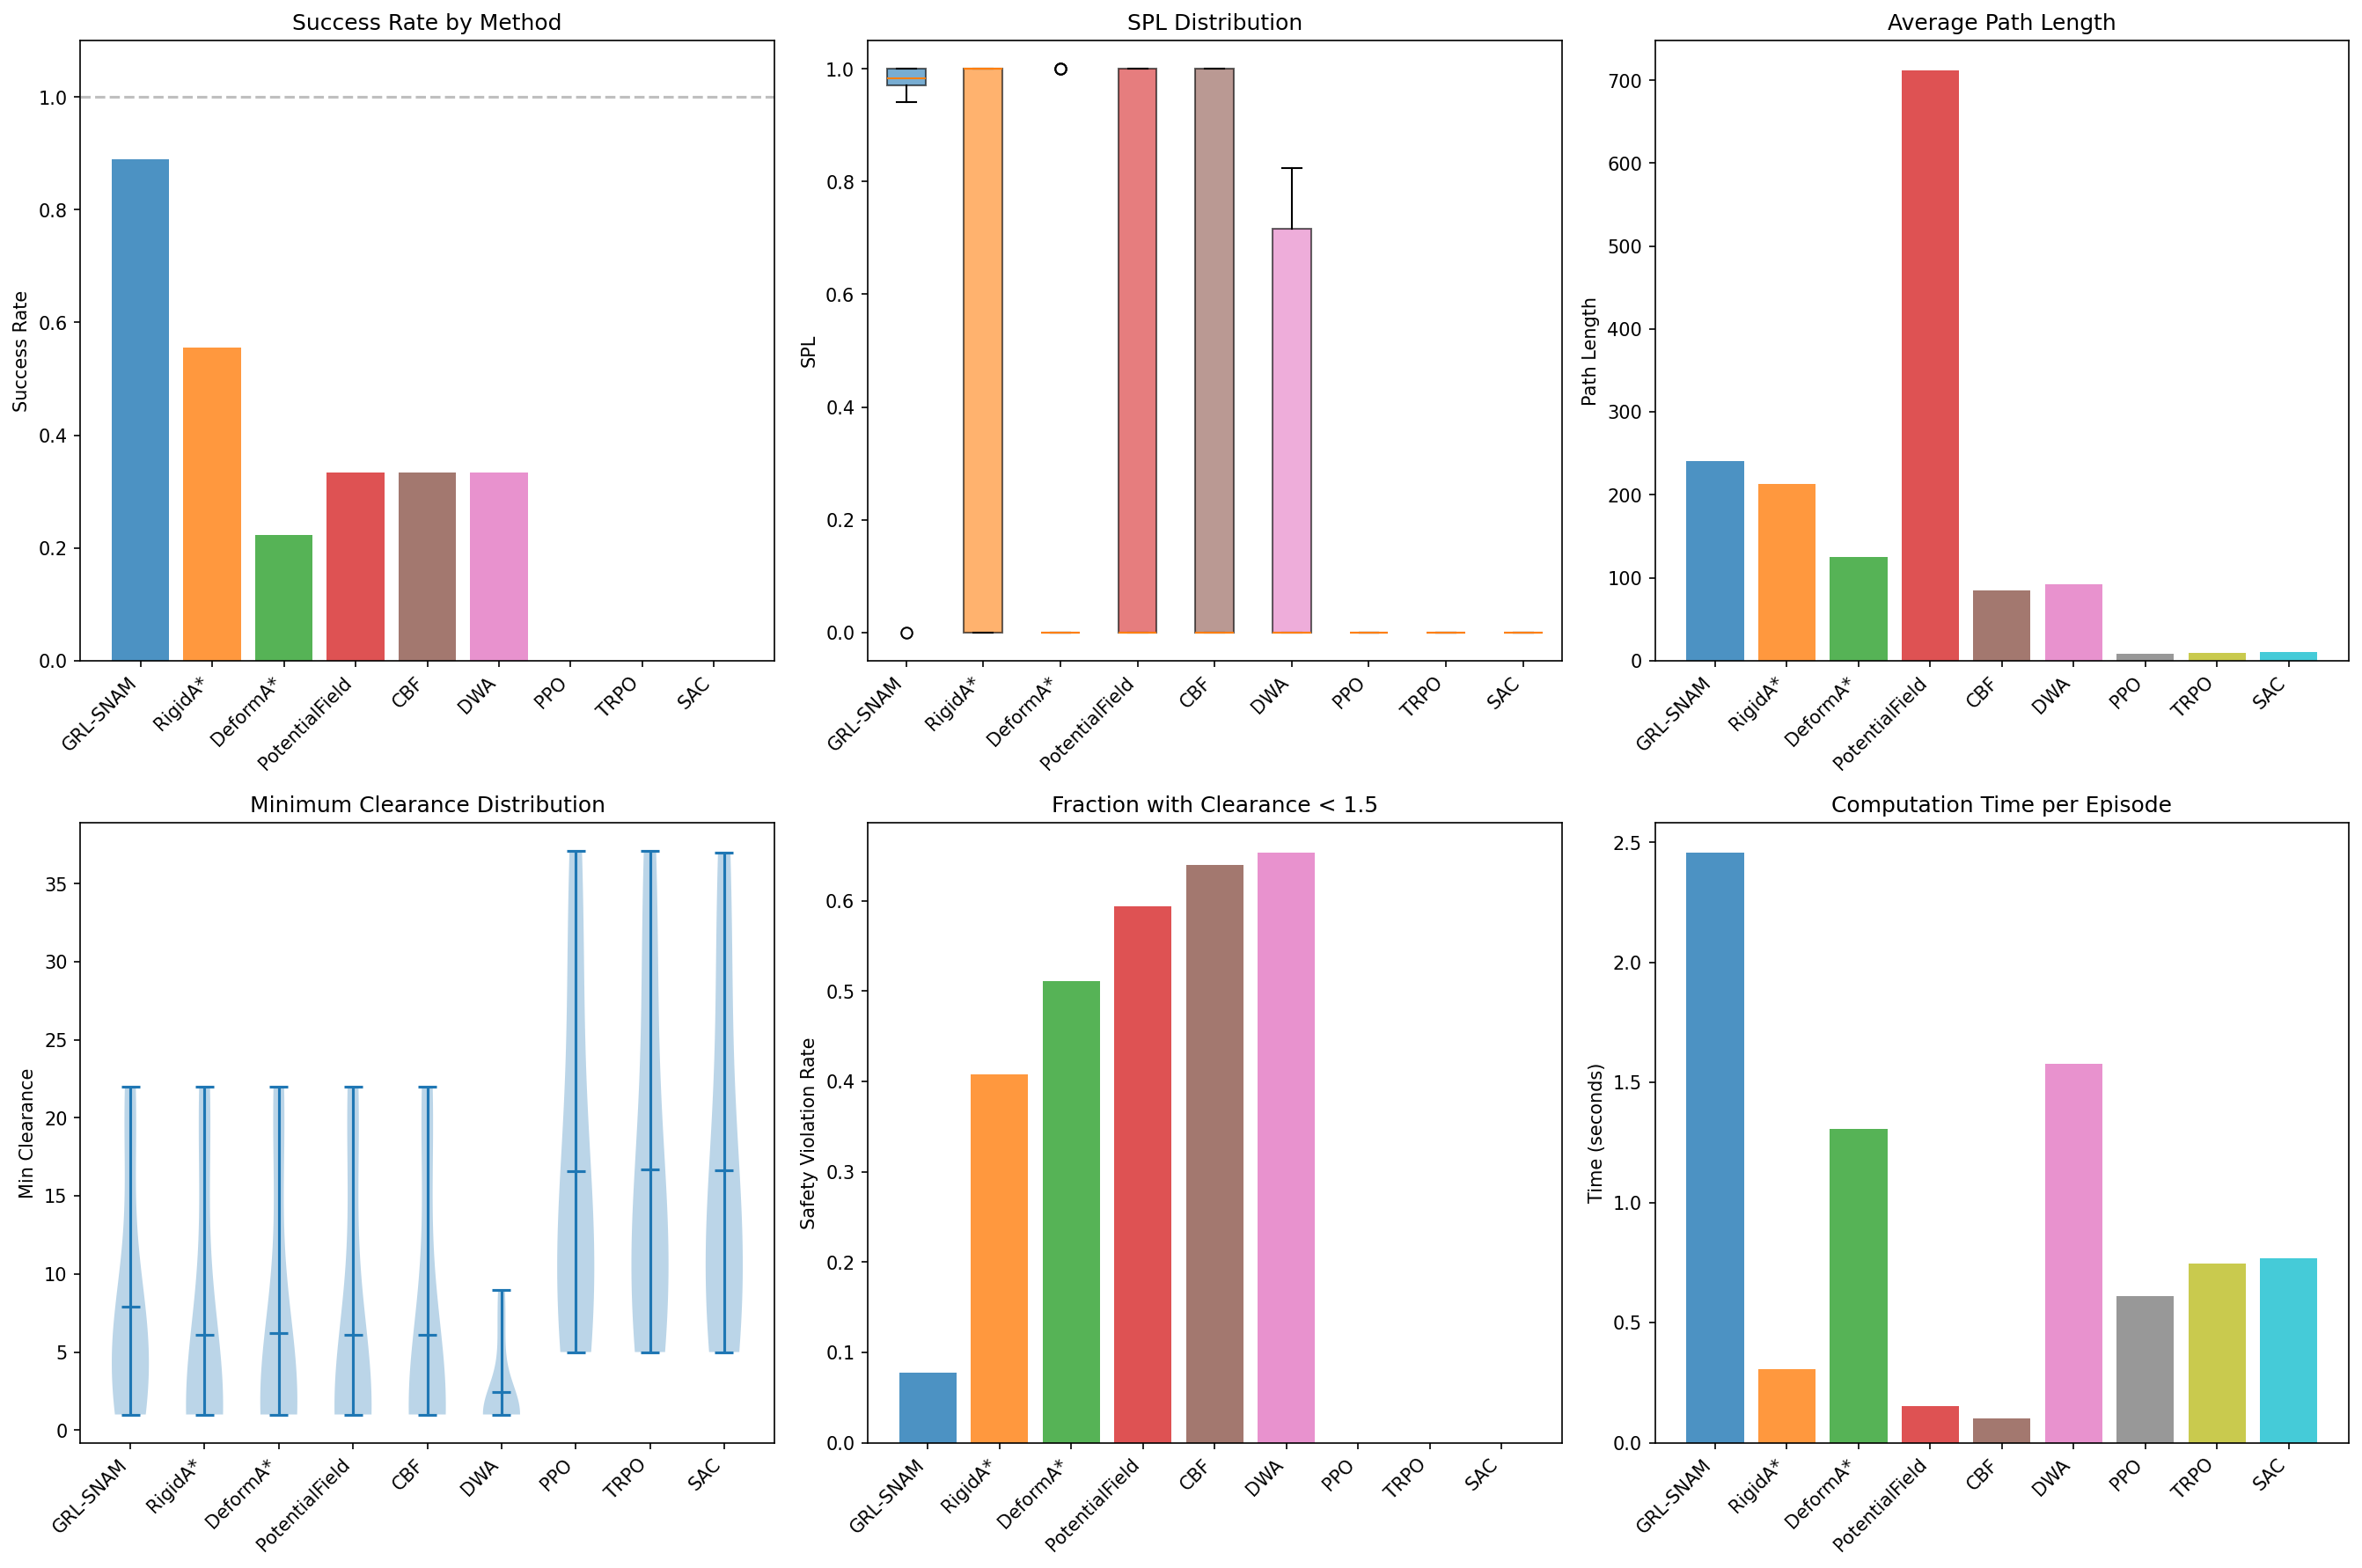
\includegraphics[width=0.48\linewidth]{AllTrials_ood.png}
    \caption{{\textbf{Test-ID (left) and Test-OOD (right) dashboard (aggregate over all trials).}
Each side contains six panels.
\emph{Top row (performance/efficiency):} (1) success rate; (2) SPL distribution (zeros correspond to failures; higher is better among successes); (3) average path length.
\emph{Bottom row (safety/cost):} (4) distribution of per-episode minimum clearance $\mathrm{clr}_{\min}=\min_n \mathrm{clr}_n$; (5) grazing rate $\mathbb{P}(\mathrm{clr}_{\min}\le d_{\text{thr}})$ with $d_{\text{thr}}{=}1.5$; (6) average computation time per episode.
GRL-SNAM achieves a strong joint trade-off across splits: high success with high SPL and short paths, while preserving positive clearance (low grazing rate) at moderate compute.}}

    \label{fig:exp1_comparison}
\end{figure}


\subsection{Learning {Strategies} in Dungeon Navigation: Deep RL vs.\ Hamiltonian Supervision}
\label{subsec:rl_baselines}

The dungeon point-agent task isolates the \emph{learning signal} under matched dynamics and observations: all methods share the same 2D continuous control, local occupancy encoding, and Transformer encoder; only the training objective differs.
We report (i) end-to-end, full-episode RL on the long-horizon MDP, and (ii) stagewise short-rollout training with the same observation/action interface used by GRL-SNAM.

\paragraph{Full-episode deep RL (long-horizon).}
We train PPO, TRPO, and SAC to reach a global goal within a 2000-step budget using only local observations.
Despite 5--8M environment transitions, success remains below 8\% and collision rates are $\sim$25\%, highlighting the difficulty of long-horizon credit assignment under partial observability.

\begin{table}[htbp]
\centering
% \caption{{\color{red} Please conclude caption with a full assesment of the success/failure of  RL methods, and also point to the dungeon figures for cross-reference of cases where success/failure occurs as visual proof.} Full-episode end-to-end navigation baselines in the dungeon environment.}
\caption[Full-episode end-to-end RL baselines in the dungeon]{
Full-episode, end-to-end navigation baselines (PPO/TRPO/SAC) in the dungeon environment.
Despite substantial training budgets (5--8M environment steps), all three RL methods
fail to learn reliable goal-directed navigation under the dungeon’s partial/local observations:
success remains extremely low (1.5--7.2\%), collisions are frequent (23.5--28.3\%), and the
agent typically terminates far from the goal (mean residual distance 14--24\,m).
See Fig.~\ref{fig:dungeon_map} for qualitative evidence.%
}
\label{tab:full_episode_rl}
\small
\begin{tabular}{lcccc}
\toprule
Algorithm & Success (\%) & Mean goal dist.\ (m) & Collision (\%) & Env.\ training steps \\
\midrule
PPO  & 7.2 & 14.1 & 23.5 & 5M \\
TRPO & 3.8 & 23.7 & 26.1 & 6.5M \\
SAC  & 1.5 & 20.2 & 28.3 & 8M \\
\bottomrule
\end{tabular}
\end{table}

\paragraph{Stagewise short-rollout RL (matched interface).}
To remove interface confounds, we train the same RL algorithms on the \emph{same} stagewise short-rollout distribution and structured observations as GRL-SNAM: stage-relative state, stage-exit goal, and locally extracted obstacles, with actions $\mathbf{a}_t=[v_x,v_y]$.
RL improves over the full-episode setting, but still plateaus well below GRL-SNAM.

\begin{table}[htbp]
\centering
\caption[Stagewise short-rollout baselines vs.\ GRL-SNAM]{
Short-rollout, stagewise baselines vs.\ GRL-SNAM on the same dungeon-derived dataset and the same sensors.
While PPO/TRPO/SAC improve over full-episode training, they remain limited in reliability
(18.4--26.1\% success) and exhibit noticeably larger tracking error and residual goal distance.
In contrast, GRL-SNAM achieves 87.5\% success with substantially lower state error and goal distance, indicating that the learned GRL-SNAM surrogate produces actions that are both locally safe and globally progress-seeking. This advantage is displayed with the qualitative comparison in Fig.~\ref{fig:dungeon_map}.%
}

\small
\begin{tabular}{lcccc}
\toprule
Algorithm & Success (\%) & Mean state error (m) $\downarrow$ & Mean goal dist.\ (m) $\downarrow$ & Env.\ training\ steps \\
\midrule
PPO      & 26.1 & 1.8 & 1.2 & $\approx 3.2$M env.\ steps \\
TRPO     & 21.7 & 2.1 & 1.5 & $\approx 3.8$M env.\ steps \\
SAC      & 18.4 & 2.4 & 1.9 & $\approx 4.1$M env.\ steps \\
GRL-SNAM & \textbf{87.5} & \textbf{0.3} & \textbf{0.1} & 500k gradient steps \\
\bottomrule
\end{tabular}
\label{tab:short_rollout_rl}
\end{table}

\paragraph{Takeaway: objective dominates optimizer.}
With dynamics, sensing, and encoder fixed, swapping PPO/TRPO/SAC changes results modestly but does not close the gap.
The consistent improvement comes from \emph{Hamiltonian-structured supervision}: GRL-SNAM learns an energy model whose gradients encode goal attraction, barrier avoidance, and dissipation, rather than optimizing a sparse scalar reward.
This yields substantially higher success and lower terminal error in the same observation/action regime, indicating that the advantage is primarily due to the learning formulation rather than the choice of RL optimizer.


\subsection{Hamiltonian Field and Constraint Learning}
\label{subsec:hamiltonian_analysis}

We analyze the learned force fields, barrier structure, and replay contents on the hyperelastic ring under stagewise sensing.

\paragraph{Force-field decomposition.}
Figure~\ref{fig:vector_fields} visualizes the learned force field (negative differential of sub-modular potentials) as
goal attraction $F_g$, obstacle barriers $F_{bs}$, and their composition
\begin{equation}
F = \beta F_g + \gamma F_{bs}.
\label{eq:force_composition}
\end{equation}
$F_g$ alone is task-directed but obstacle-agnostic, while $F_{bs}$ encodes avoidance without a navigation objective.
Their composition produces smooth, clearance-preserving arcs around clutter via adaptive reweighting through $(\beta,\gamma)$.

\begin{figure}[htbp]
    \centering
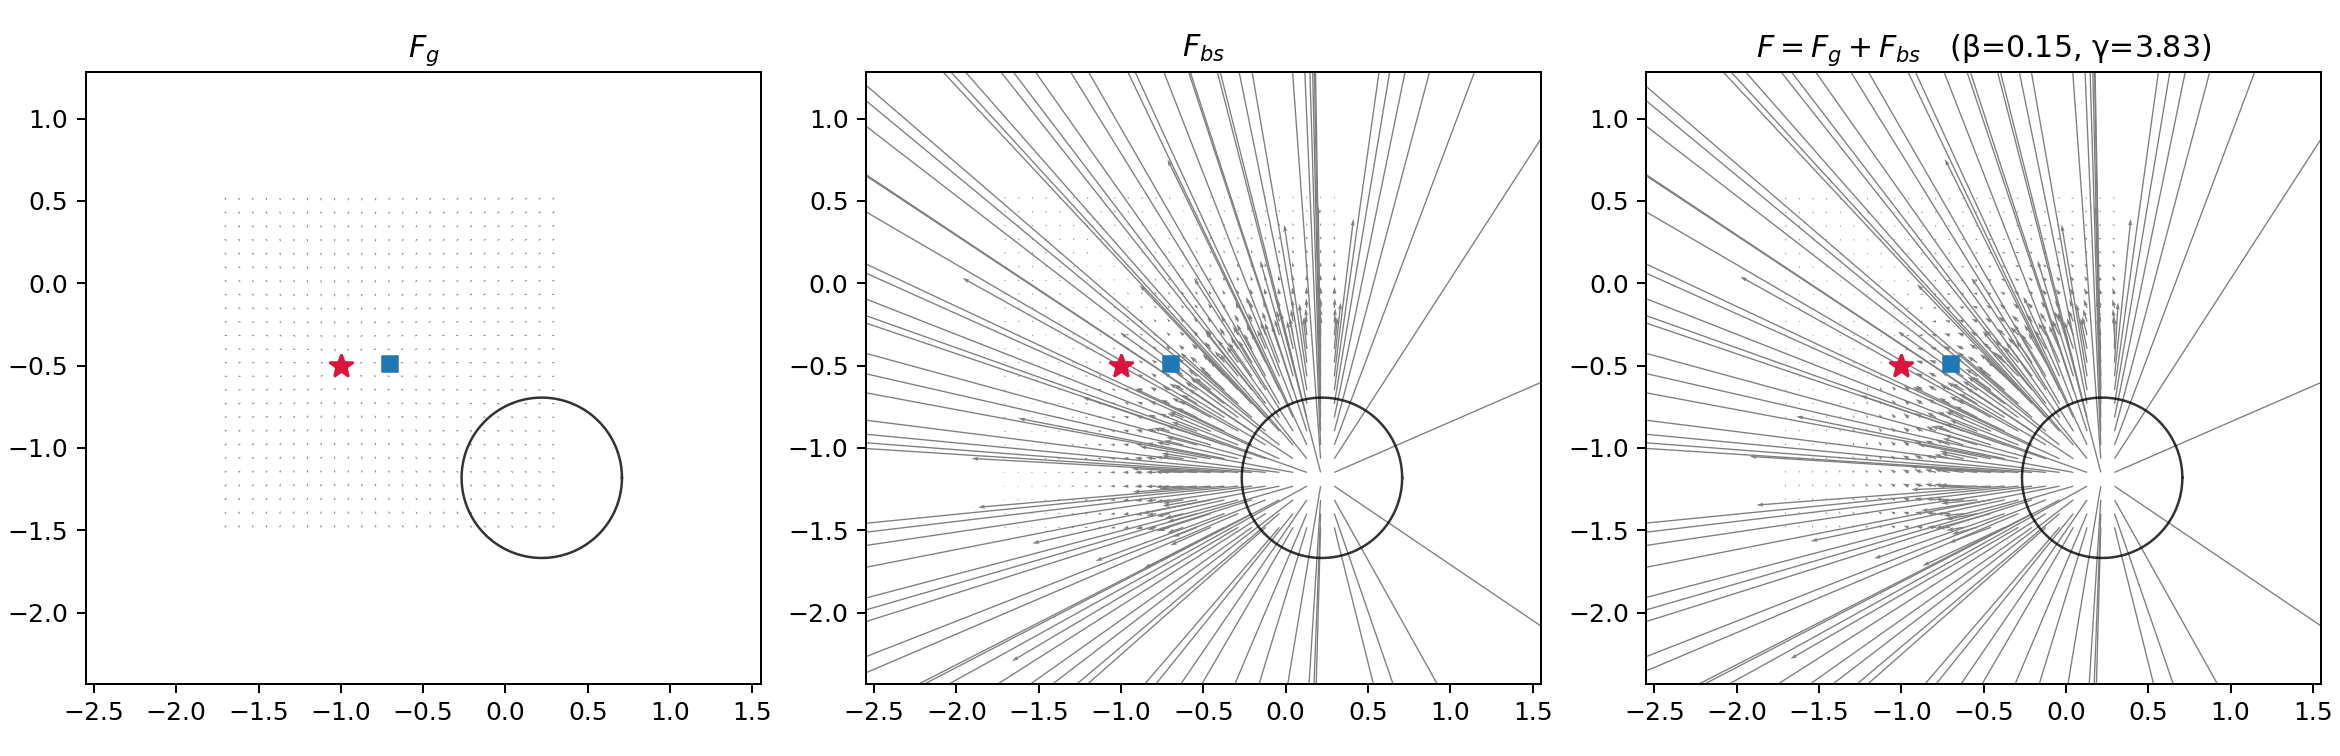
\includegraphics[width=0.8\textwidth]{vector_fields_example.png}
\caption{\textbf{Learned Hamiltonian field decomposition.}
Shown are the constituent fields used by GRL-SNAM to generate local motion under partial, stagewise observations.
\textbf{Left:} $F_g$ points toward the current stage goal and captures progress, but ignores obstacles.
\textbf{Middle:} $F_{bs}$ is induced by locally sensed barriers and encodes avoidance/clearance, but lacks task direction.
\textbf{Right:} the deployed field $F=\beta F_g+\gamma F_{bs}$ combines both effects; the learned, context-dependent coefficients $(\beta,\gamma)$ modulate the relative strength of goal following vs.\ obstacle avoidance, producing a trajectory direction that threads the corridor while maintaining a safety margin near contact regions.}
\label{fig:vector_fields}
\end{figure}

\paragraph{Online coefficient adaptation.}
Along a representative rollout (Fig.~\ref{fig:time_series}), clearance decreases near bottlenecks and recovers after passage (top).
The magnitudes $|F_g|$ and $|F_{bs}|$ rebalance accordingly (middle), while coefficients $(\beta,\gamma,\alpha)$ vary smoothly over time (bottom), indicating adaptation occurs through the Hamiltonian parametrization rather than ad hoc action scaling.

\begin{figure}[htbp]
    \centering
    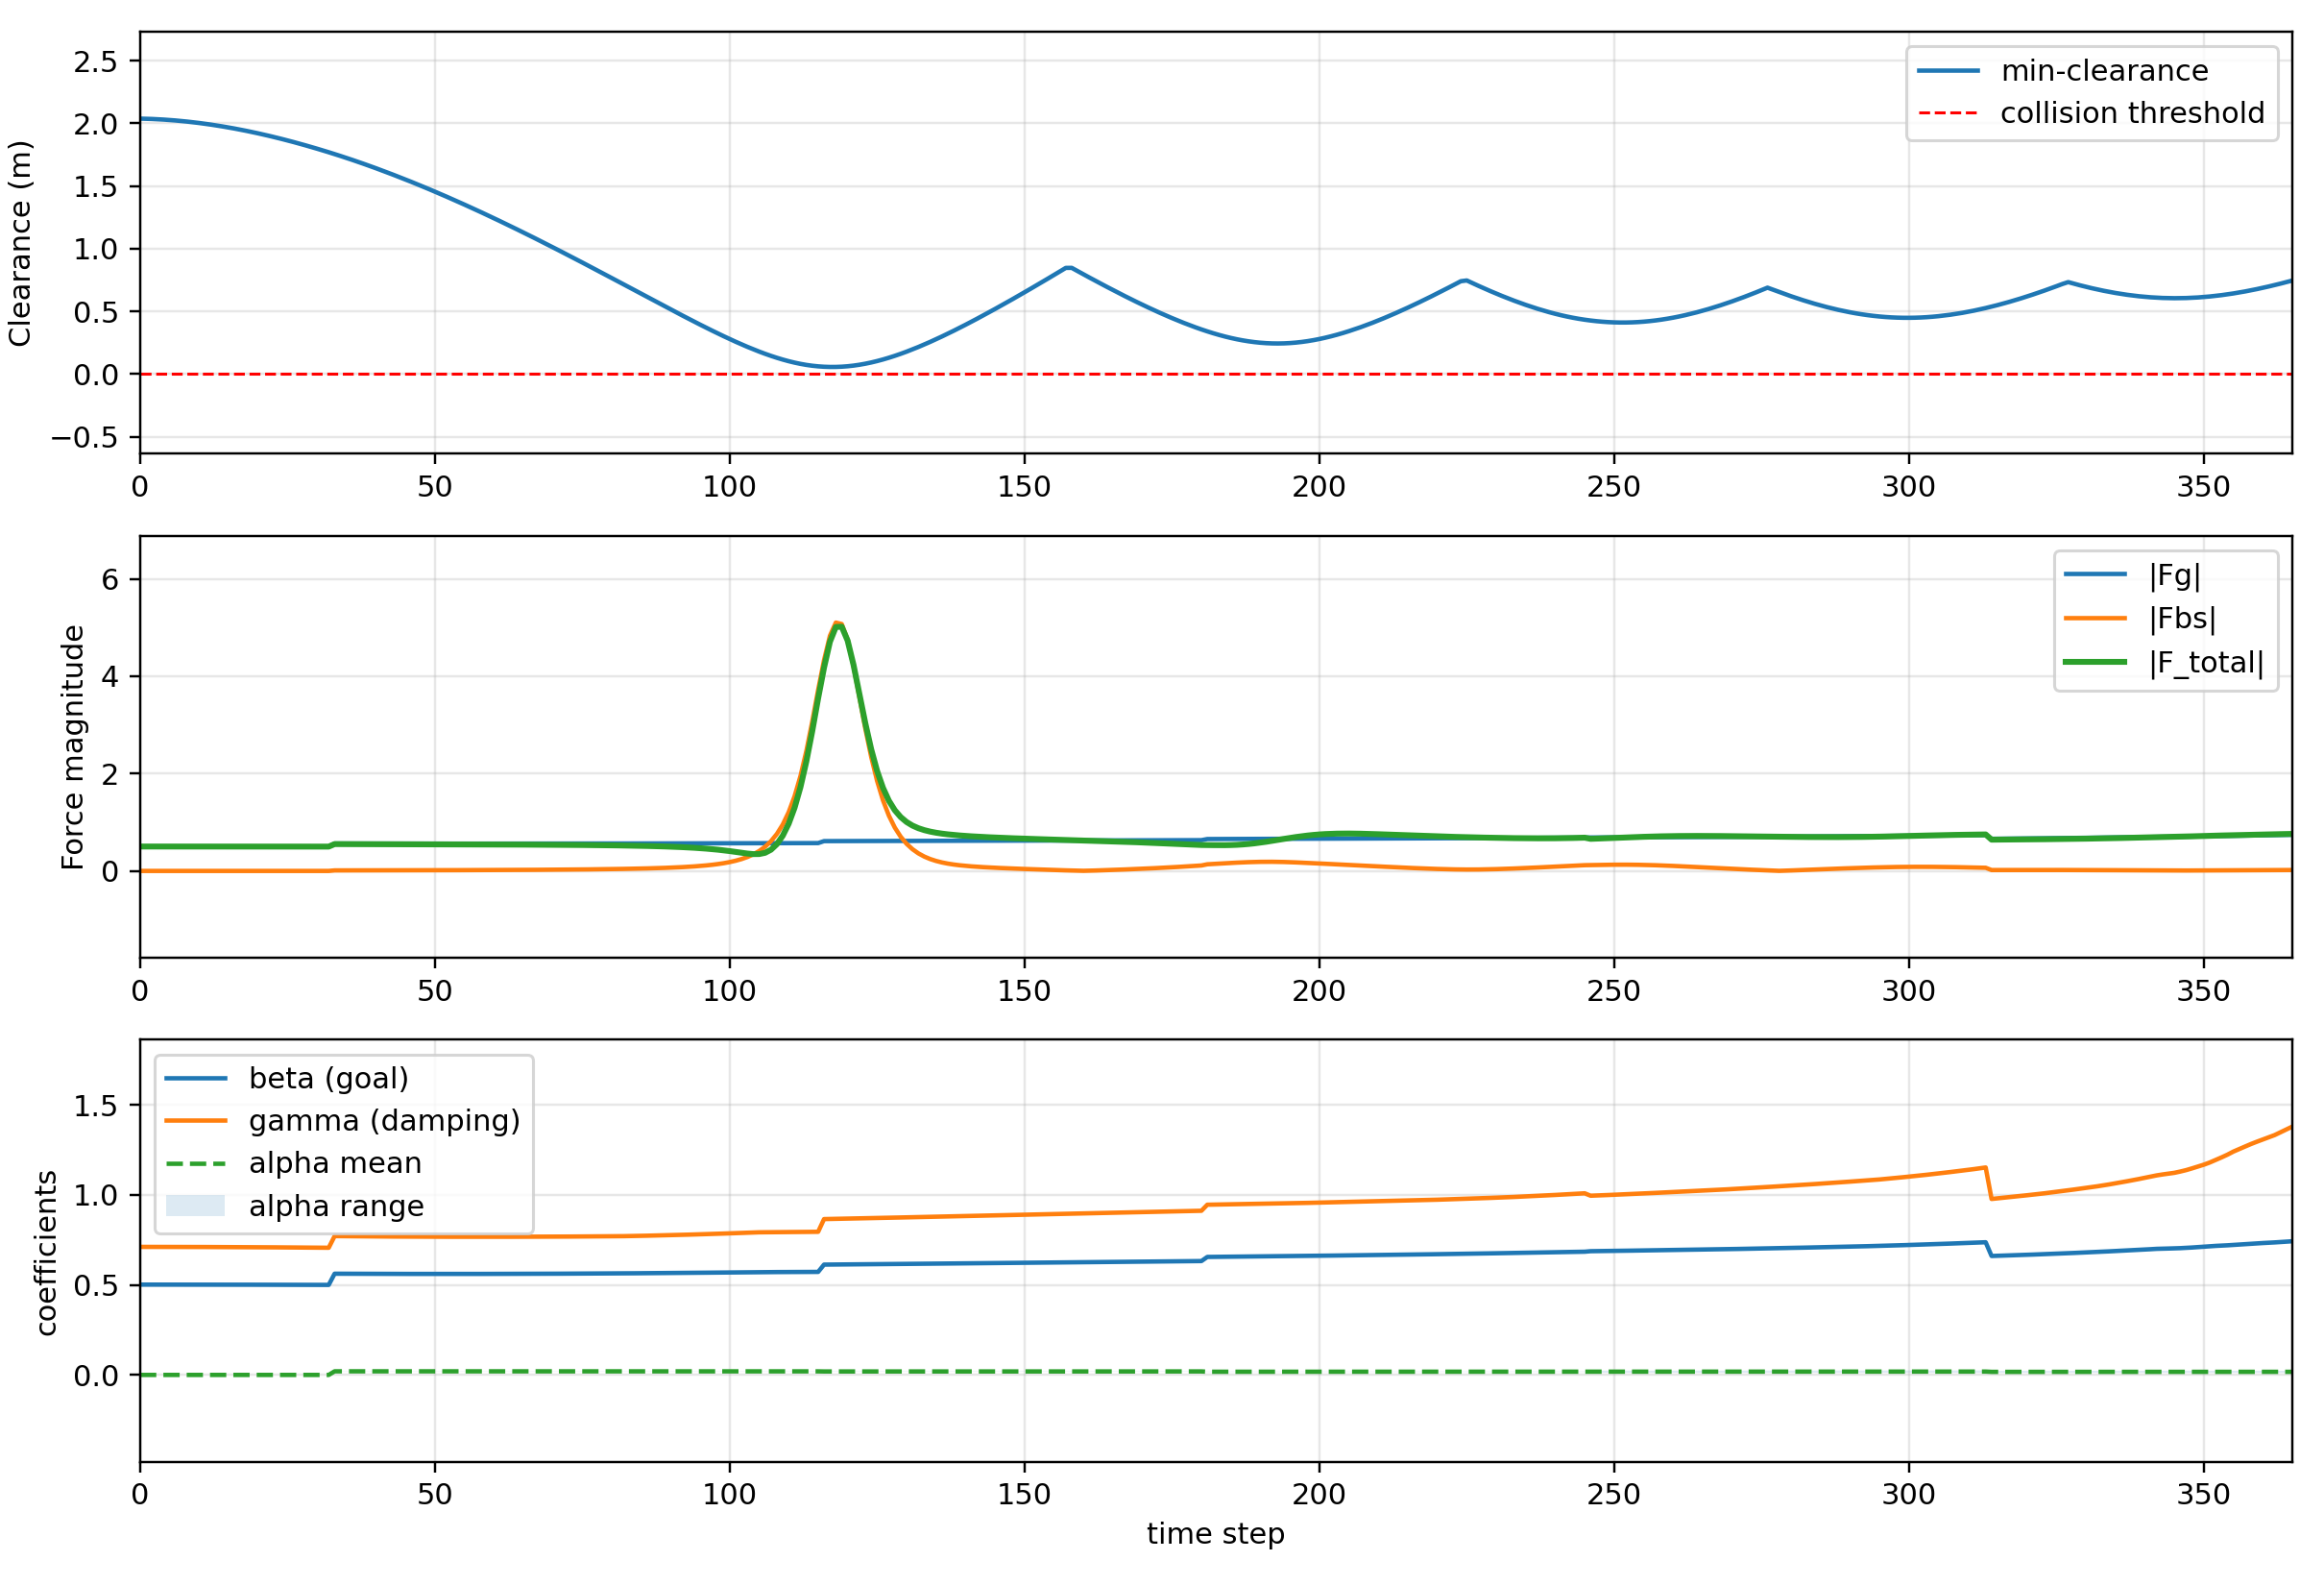
\includegraphics[width=0.6\textwidth]{timeseries_forces_clearance_coeffs.png}
    \caption{\textbf{Temporal analysis of Hamiltonian adaptation.}
    Top: minimum clearance. Middle: $|F_g|$ and $|F_{bs}|$. Bottom: coefficients $(\beta,\gamma,\alpha)$.
    Coefficients change smoothly as the robot enters/exits clutter, rebalancing goal and barrier terms.}
    \label{fig:time_series}
\end{figure}

\paragraph{Empirical barrier learning.}
Figure~\ref{fig:barrier_profile} compares the learned obstacle barrier energy to the simulator’s analytic reference using an angle-averaged radial profile.
The learned barrier is near-zero at large clearance and rises sharply near contact, closely tracking the reference while slightly softening at intermediate distances and steepening near contact, consistent with additional deformation/friction costs captured in the rollout data.

\begin{figure}[htbp]
    \centering
    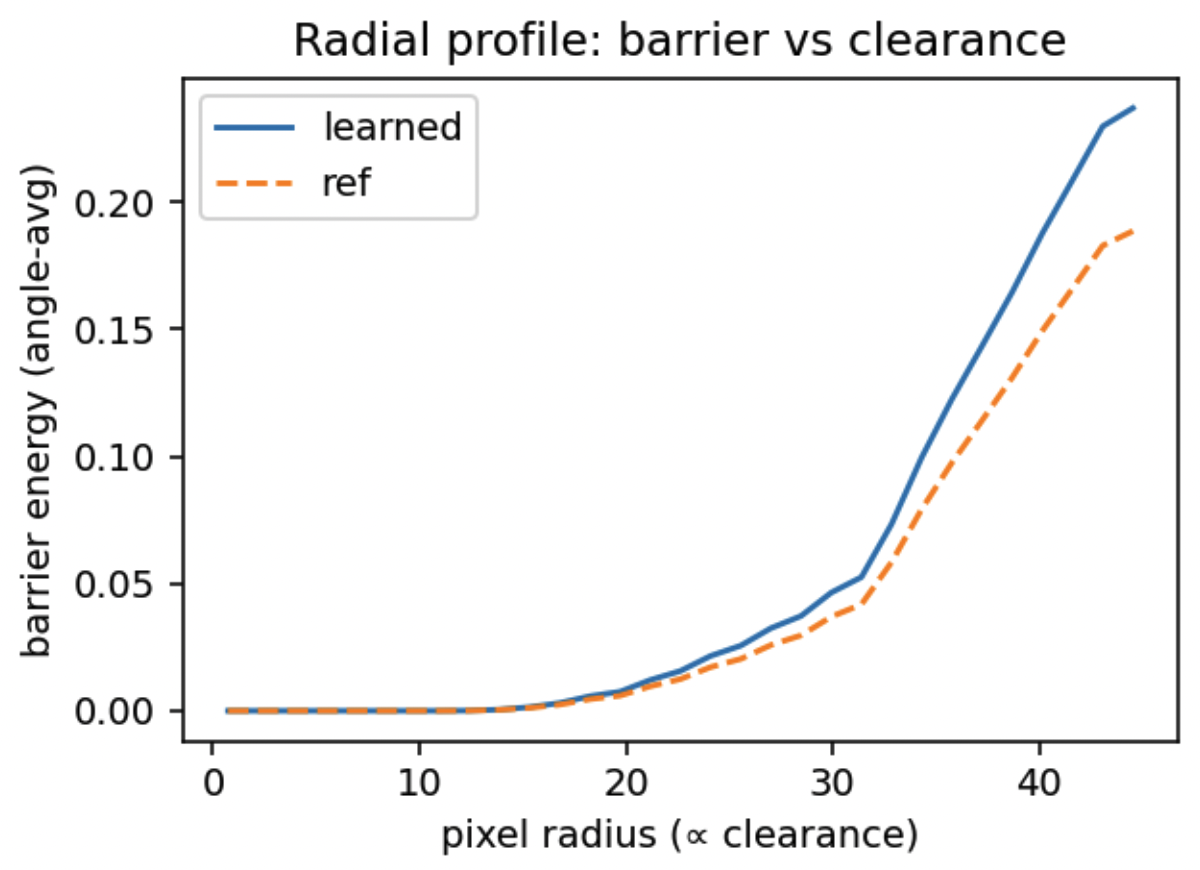
\includegraphics[width=0.55\textwidth]{barrier_radial_profile.png}
    \caption{\textbf{Radial profile of barrier energy vs.\ clearance.}
    Angle-averaged barrier energy around obstacles for the learned barrier (solid) and analytic reference (dashed).
    The learned profile matches the reference trend and sharpens near contact. { The difference between two curves indicates Our method can learn to adapt the energy landscape based on its current environment context.}}
    \label{fig:barrier_profile}
\end{figure}

\paragraph{Stagewise reuse and bootstrapped refinement.}
Stagewise parameterization induces a family of local policies (sensor/frame/shape controllers) that share parameters but adapt $(\beta,\gamma,\alpha)$ by stage.
As new windows are visited, local rollouts refine the Hamiltonian for those regions; revisits exploit this refinement without recomputing global plans.
Empirically, trajectories tighten toward least-cost paths over time while maintaining positive clearance.

\paragraph{Replay buffer thriftiness.}
Figure~\ref{fig:replay_buffer} shows buffer memory is dominated by local transitions $(q_t,q_{t+1})$ (about 80\%), with compact constraint/contact summaries (about 15\%); actions, gradients, barrier scales, and rewards occupy only a few percent.
The buffer therefore stores only what is needed for Hamiltonian updates—local dynamics and local constraints—without caching full maps or dense cost volumes.

\begin{figure}[htbp]
    \centering
    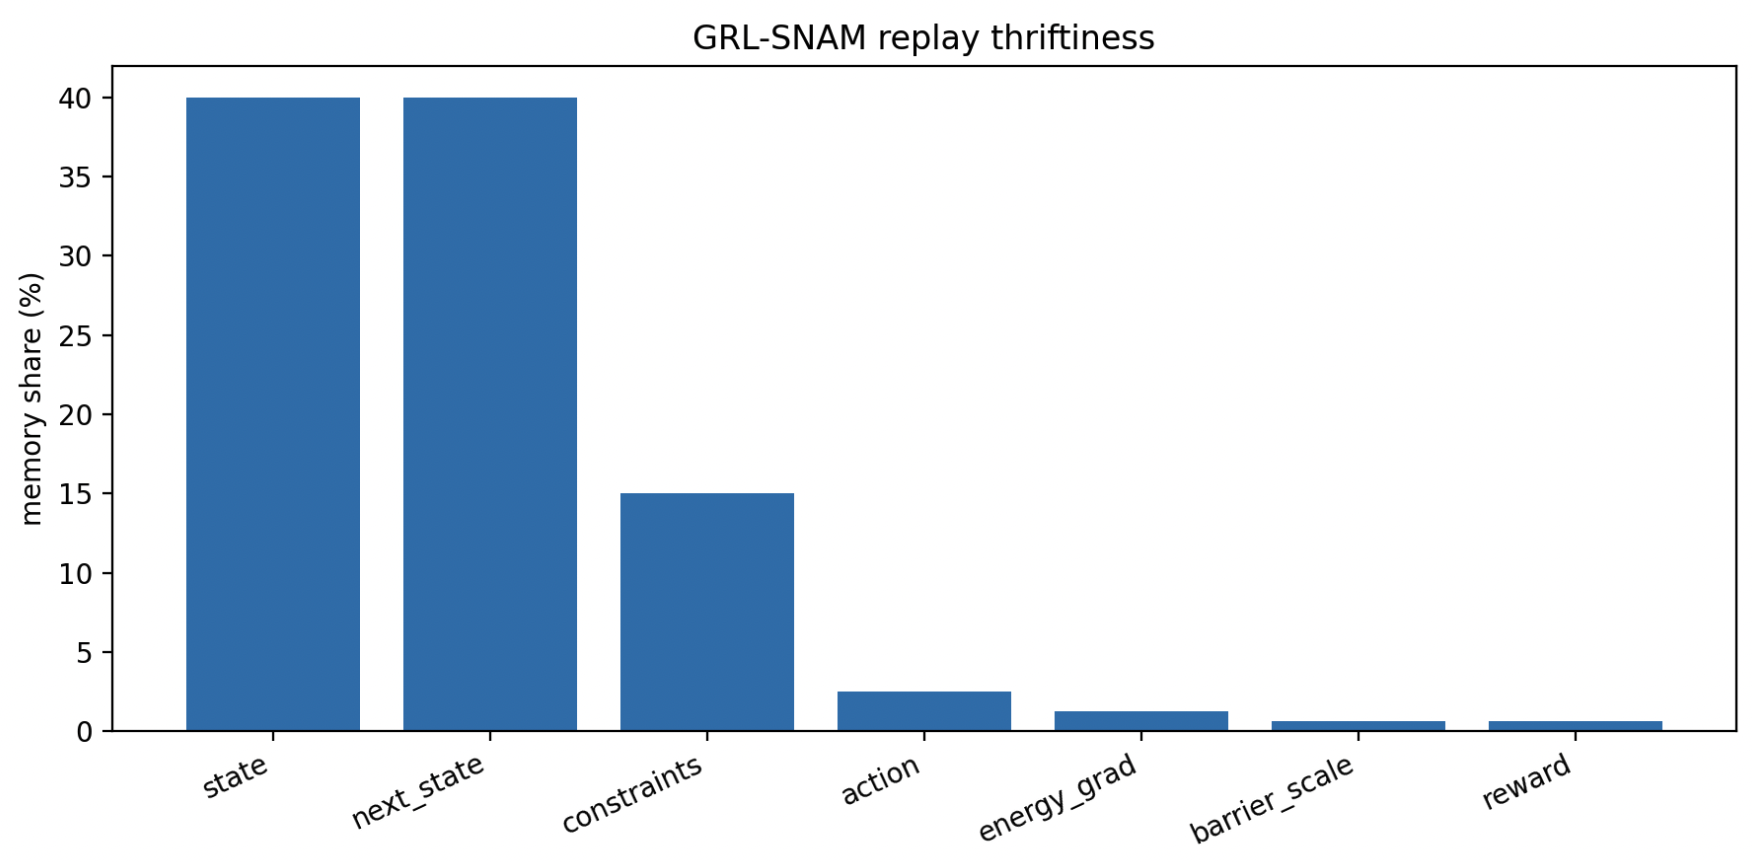
\includegraphics[width=0.75\linewidth]{replay_thriftiness.png}
    \caption{\textbf{Replay thriftiness in GRL-SNAM.}
    Memory share of buffer fields: $\sim$80\% local transitions $(q_t,q_{t+1})$, $\sim$15\% compact constraint/contact sets, and only a few percent for actions, gradients, barrier scales, or rewards. { GRL-SNAM is memory efficient as it only maintains the local state exhaustively while using a low dimensional network structure which effectively encodes the energy landscape.}}
    \label{fig:replay_buffer}
\end{figure}

\paragraph{Closed-loop Hamiltonian refinement.}
Stagewise interaction supplies short rollouts that populate the buffer (Fig.~\ref{fig:replay_buffer});
buffer updates adjust coefficients and barrier parameters, reshaping the local landscape (Figs.~\ref{fig:vector_fields}--\ref{fig:barrier_profile});
the updated landscape then induces the next round of dynamics.
This yields a closed-loop procedure that repeatedly refines $\mathcal{H}_\theta$ from local experience.


\subsection{Ablations and Robustness}
\label{subsec:ablations_robustness}

We finally probe how specific design choices in GRL-SNAM affect performance, and how well the learned Hamiltonian controller tolerates sensing and dynamics perturbations.

\paragraph{Effect of loss components.}
Recall that our navigation surrogate is trained with a weighted multi-term loss
\begin{equation}
\mathcal{L} = w_{\text{traj}} \mathcal{L}_{\text{traj}} + w_{\text{vel}} \mathcal{L}_{\text{vel}} + w_{\text{friction}} \mathcal{L}_{\text{friction}} + w_{\text{multi}} \mathcal{L}_{\text{multi}},
\label{eq:total_loss}
\end{equation}
where $\mathcal{L}_{\text{traj}}$ and $\mathcal{L}_{\text{vel}}$ supervise trajectory and velocity matching, $\mathcal{L}_{\text{friction}} = \|\gamma - \gamma_o\|_2^2$ aligns the learned damping with the stagewise reference, and $\mathcal{L}_{\text{multi}}$ trains near-contact robustness via perturbed short rollouts.
We ablate the last two terms while keeping environments and architectures fixed.

\begin{table}[htbp]
\centering
\caption{\textbf{Ablation of loss terms} on the hyperelastic ring benchmark (Test-ID/OOD).
Arrows denote desired direction. Icons summarize consistent qualitative trends across several seeds.}
\small
\setlength{\tabcolsep}{6pt}
\begin{adjustbox}{valign=c, width=\textwidth}
\begin{tabular}{lcccccc}
\toprule
\textbf{Variant} & \textbf{Collisions} $\downarrow$ & \textbf{MinClr} $\uparrow$ & \textbf{Barrier Viol.} $\downarrow$ & \textbf{Progress/SPL} $\uparrow$ & \textbf{Smoothness} $\downarrow$ & \textbf{Observed behavior}\\
\midrule
$w_{\text{fric}} = 0,\ w_{\text{multi}} = 0$    & \textcolor{red}{High} ($\times$) & \textcolor{red}{$<0$} & \textcolor{red}{High} & \textcolor{red}{Poor} & \textcolor{red}{Poor} & Penetrates obstacles \\
$w_{\text{fric}} = 0,\ w_{\text{multi}} = 0.5$   & \textcolor{green!50!black}{Low}~($\checkmark$) & \textcolor{green!50!black}{High} & \textcolor{green!50!black}{Low} & \textcolor{orange}{Low} & \textcolor{green!50!black}{OK} & Very slow, conservative \\
$w_{\text{fric}} = 0.1,\ w_{\text{multi}} = 0$   & \textcolor{green!50!black}{None}~(\checkmark) & \textcolor{green!50!black}{High} & \textcolor{green!50!black}{Low} & \textcolor{green!50!black}{High} & \textcolor{green!50!black}{Best} & Smooth, stable, fast \\
$w_{\text{fric}} = 0.1,\ w_{\text{multi}} = 0.5$ & \textcolor{green!50!black}{None}~($\checkmark$) & \textcolor{orange}{Slightly lower} & \textcolor{green!50!black}{Low} & \textcolor{green!50!black}{High} & \textcolor{green!50!black}{Good} & Stable; tighter margins \\
\bottomrule
\end{tabular}
\end{adjustbox}

\label{tab:ablation_fric_multi}
\end{table}

Table~\ref{tab:ablation_fric_multi} shows that:
(i) without $\mathcal{L}_{\text{friction}}$ or $\mathcal{L}_{\text{multi}}$, the learned field is under-damped and oscillatory, leading to barrier violations and penetrations;
(ii) $\mathcal{L}_{\text{multi}}$ alone enforces safety but at the cost of extremely slow motion, as the learner over-weights near-contact failures and suppresses progress;
(iii) $\mathcal{L}_{\text{friction}}$ alone is sufficient to eliminate penetrations and produce smooth, fast trajectories; and
(iv) combining both terms yields the best overall trade-off, with slightly tighter clearances but robust, stable motion in clutter.
These trends are consistent with the Hamiltonian interpretation: $\mathcal{L}_{\text{friction}}$ learns an appropriate dissipation term, preventing “ringing’’ of the barrier energy, while $\mathcal{L}_{\text{multi}}$ selectively shapes the field near constraints.

\paragraph{Robustness to sensing and dynamics perturbations.}
We next evaluate GRL-SNAM under controlled perturbations to sensing and dynamics.
We vary position jitter and radius estimation error in the local obstacle extractor, randomly drop or hallucinate obstacles, and perturb the damping coefficient $\gamma$ and applied velocities.
Each start–goal pair is rolled out across a grid of perturbation levels, yielding a total of $N = n_{\text{env}} \times n_{\text{trials}} \times n_{\text{perturbations}}$ runs.

\begin{table}[htbp]
\centering
\caption{Robustness of GRL-SNAM to sensing noise and dynamics perturbations.
Perturbation settings are reported as (sensing noise, damping scale). { Even when noise level in sensor and motion is very high (Severe Noise), our method is still robust and achieve 87\% overall success rate, which is better comparing against RL methods.}}
\label{tab:robustness}
\vspace{0.5em}
\begin{tabular}{lcccc}
\toprule
Perturbation Level & Success (\%) & SPL $\uparrow$ & Min. Clearance (m) $\uparrow$ & Collisions $\downarrow$ \\
\midrule
Nominal (0.0, 1.0)      & 98.7 & 0.82 & 0.36 & 0.3 \\
Mild Noise (0.05, 0.9)  & 91.3 & 0.79 & 0.33 & 0.7 \\
Severe Noise (0.10, 0.7) & 87.1 & 0.72 & 0.29 & 1.1 \\
\bottomrule
\end{tabular}
\end{table}

As shown in Table~\ref{tab:robustness}, GRL-SNAM maintains high success rates ($\geq 87\%$) and positive clearance even under severe noise and dynamics mismatch.
SPL and clearance degrade gracefully as perturbations increase, while collision counts remain low.
Rather than failing catastrophically when constraints or dynamics are mis-specified, the learned Hamiltonian field re-weights goal and barrier terms in response to distorted local observations (cf.\ Figure~\ref{fig:time_series}), preserving a meaningful safety–progress trade-off.

\paragraph{Takeaways.}
The performance of
(i) the friction and multi-start losses play distinct, interpretable roles in learning dissipation and near-contact robustness in the Hamiltonian surrogate;
(ii) performance is not brittle to moderate changes in sensing or dynamics, because GRL-SNAM adapts by reshaping the energy landscape rather than overfitting to a single nominal model; and
(iii) these properties are emergent from the same empirical Hamiltonian-modification pipeline analyzed in Section~\ref{subsec:hamiltonian_analysis}, reinforcing our claim that GRL-SNAM provides a stable, constraint-aware alternative to standard reward-based policies for stagewise navigation.

